% ============================================================================
% Dissertation: Personalized Privacy-Preserving Split Learning (P3SL)
% with a Bi-Level Utility-Constrained Differential-Privacy Loop.
%
% Build (Tectonic, no external bibtex needed; uses thebibliography environment):
% tectonic thesis.tex
% Or pdflatex (3 passes):
% pdflatex thesis.tex && pdflatex thesis.tex && pdflatex thesis.tex
% ============================================================================
\documentclass[11pt,a4paper,oneside]{report}

\usepackage[T1]{fontenc}
\usepackage[utf8]{inputenc}
\usepackage{lmodern}
\usepackage[a4paper,margin=1in,headheight=14pt]{geometry}
\usepackage{microtype}
\usepackage{amsmath,amssymb,amsfonts}
\renewcommand{\bibname}{References}
\usepackage{graphicx}
\usepackage{booktabs}
\usepackage{multirow}
\usepackage{array}
\usepackage{xcolor}
\usepackage{url}
\usepackage{enumitem}
\usepackage{titlesec}
\usepackage{fancyhdr}
\usepackage{setspace}
\usepackage{algorithm}
\usepackage{algpseudocode}
\usepackage{hyperref}
\hypersetup{
 colorlinks=true,
 linkcolor=black,
 citecolor=blue,
 urlcolor=blue,
 pdftitle={Personalized Privacy-Preserving Split Learning with a
 Bi-Level Utility-Constrained Differential-Privacy Loop},
 pdfauthor={Yogesh Kumar; Vikhyat Charak; Paras},
 pdfsubject={Split Learning; Differential Privacy; Federated Learning;
 Reconstruction Attacks; Membership Inference; Backdoors},
 pdfkeywords={split learning, differential privacy, federated learning,
 reconstruction attack, membership inference, backdoor, FashionMNIST,
 bi-level optimisation, RDP accountant, personalisation}
}

%; DTU departmental header for Declaration and Certificate pages ----------
\newcommand{\dtuheader}{%
\noindent\begin{tabular}{@{}m{0.20\textwidth}@{\hspace{0.04\textwidth}}m{0.71\textwidth}@{}}
\centering
\includegraphics[width=0.75\linewidth]{figures/dtu_crest.png} &
\centering
{\large\bfseries DEPARTMENT OF COMPUTER SCIENCE AND ENGINEERING}\\[2pt]
{\large\bfseries DELHI TECHNOLOGICAL UNIVERSITY}\\[2pt]
{(Formerly Delhi College of Engineering)}\\[2pt]
{Bawana Road, Delhi--110042}\tabularnewline
\end{tabular}%
\vspace{1.8em}\par
}

\onehalfspacing

%; Header / footer ---------------------------------------------------------
\pagestyle{fancy}
\fancyhf{}
\fancyhead[L]{\nouppercase{\leftmark}}
\fancyhead[R]{\thepage}
\renewcommand{\headrulewidth}{0.3pt}

%; Chapter heading styling -------------------------------------------------
\titleformat{\chapter}[display]
 {\normalfont\bfseries\Large\filcenter}
 {\MakeUppercase{\chaptertitlename}~\thechapter}
 {0.5em}
 {\Huge}

%; Better justification spacing --------------------------------------------
\sloppy
\emergencystretch=2em

% ============================================================================
\begin{document}

% ----------------------------------------------------------------------------
% Title page
% ----------------------------------------------------------------------------
\begin{titlepage}
\centering
\thispagestyle{empty}

\vspace*{0.2cm}
{\bfseries\large Personalized Privacy-Preserving Split Learning\\
with a Bi-Level Utility-Constrained\\
Differential-Privacy Loop\par}

\vspace{0.9cm}
{\normalsize B.TECH PROJECT-II REPORT\par}

\vspace{0.4cm}
{\normalsize SUBMITTED IN PARTIAL FULFILMENT OF THE REQUIREMENTS\\
FOR THE AWARD OF THE DEGREE\\
OF\par}

\vspace{0.4cm}
{\normalsize BACHELOR OF TECHNOLOGY\\
IN\\
\textbf{COMPUTER ENGINEERING}\par}

\vspace{0.5cm}
{\normalsize Submitted By:\\[2pt]
\textbf{Yogesh Kumar} (2K22/CO/520)\\[2pt]
\textbf{Vikhyat Charak} (2K22/CO/496)\\[2pt]
\textbf{Paras} (2K22/CO/319)\par}

\vspace{0.45cm}
{\normalsize Under the supervision of\\[2pt]
\textbf{Dr Nemalikanti Anand}\\[2pt]
(Department of Computer Science and Engineering)\par}

\vspace{0.45cm}

\includegraphics[width=0.17\textwidth]{figures/dtu_crest.png}

\vspace{0.45cm}
{\normalsize\bfseries DEPARTMENT OF COMPUTER SCIENCE AND ENGINEERING\\
DELHI TECHNOLOGICAL UNIVERSITY\par}
{\normalsize (Formerly Delhi College of Engineering)\\
Bawana Road, Delhi -- 110042\\[3pt]
\textbf{May 2026}\par}
\end{titlepage}

% ----------------------------------------------------------------------------
% Front-matter page numbering
% ----------------------------------------------------------------------------
\pagenumbering{roman}
\pagestyle{plain}

% ----------------------------------------------------------------------------
% Candidate's Declaration
% ----------------------------------------------------------------------------
\clearpage
\phantomsection
\addcontentsline{toc}{chapter}{Candidate's Declaration}
\thispagestyle{plain}
\markboth{Candidate's Declaration}{Candidate's Declaration}

\dtuheader

\begin{center}{\Large\bfseries CANDIDATE'S DECLARATION}\end{center}
\vspace{1em}

We, \textbf{Yogesh Kumar (2K22/CO/520), Vikhyat Charak (2K22/CO/496),
Paras (2K22/CO/319)}, pursuing Bachelor of Technology degree in
\textbf{Computer Engineering} from the Department of Computer Science
and Engineering, hereby declare that the B.\,Tech.\ Project-II report
titled \textit{``Personalized Privacy-Preserving Split Learning with a
Bi-Level Utility-Constrained Differential-Privacy Loop''} submitted by
us to the Department of Computer Science and Engineering, Delhi
Technological University, Delhi, in partial fulfilment of the degree,
is entirely original and not copied from any source without proper
citation. We hereby declare that this work has not been submitted in
part or full for any degree or diploma to this University or
elsewhere.

\vspace{2em}
\begin{flushright}
(Signature)\\
Yogesh Kumar (2K22/CO/520)\\[1.2em]
(Signature)\\
Vikhyat Charak (2K22/CO/496)\\[1.2em]
(Signature)\\
Paras (2K22/CO/319)
\end{flushright}

\vspace{1em}
\noindent Place: New Delhi\\
Date:

\clearpage

% ----------------------------------------------------------------------------
% Certificate
% ----------------------------------------------------------------------------
\clearpage
\phantomsection
\addcontentsline{toc}{chapter}{Certificate}
\thispagestyle{plain}
\markboth{Certificate}{Certificate}

\dtuheader

\begin{center}{\Large\bfseries CERTIFICATE}\end{center}
\vspace{1em}

This is to certify that the B.\,Tech.\ Project-II report entitled
\textit{``Personalized Privacy-Preserving Split Learning with a
Bi-Level Utility-Constrained Differential-Privacy Loop''} submitted by
\textbf{Yogesh Kumar (2K22/CO/520), Vikhyat Charak (2K22/CO/496), Paras
(2K22/CO/319)}, of the Department of Computer Science and Engineering,
Delhi Technological University, in partial fulfilment of the
requirement for the project work, has been carried out by the students
under my supervision. To the best of my knowledge, this work has not
been submitted in part or full for any degree or diploma to this
University or elsewhere.

\vspace{6em}
\begin{flushright}
(Signature)\\[2pt]
\textbf{Dr Nemalikanti Anand}\\
Department of Computer Science and Engineering\\
Delhi Technological University, Delhi
\end{flushright}

\vspace{1em}
\noindent Place: New Delhi\\
Date:

\clearpage

% ----------------------------------------------------------------------------
% Acknowledgements
% ----------------------------------------------------------------------------
\clearpage
\phantomsection
\addcontentsline{toc}{chapter}{Acknowledgements}
\thispagestyle{plain}
\markboth{Acknowledgements}{Acknowledgements}

\vspace*{1em}
\begin{center}{\Large\bfseries ACKNOWLEDGEMENTS}\end{center}
\vspace{1em}

This work is the result of many months of reading, prototyping
and quiet revision, and it would not exist without the people who made
the time and the space for it.

We are grateful to the Head of the Department of Computer Science and
Engineering, Delhi Technological University, for the academic
environment in which this project was carried out, and for the
periodic review meetings that helped us course-correct early when
methodological issues surfaced.

We owe the deepest thanks to our project supervisor,
\textbf{Dr Nemalikanti Anand}, whose technical direction kept this work
focused on questions that matter. Several of the more careful choices
in this report (to abandon a flashy but unfaithful evaluation
protocol, to add a formal privacy accountant when an empirical proxy
would have sufficed, to insist on multi-seed reporting) were made in
response to that feedback.

We thank the faculty of the Department of Computer Science and
Engineering for the coursework on which this work builds, the
open-source maintainers of the libraries we relied on, and our
families and peers for their patience over the long hours of
debugging, plotting and rewriting.

\vspace{2em}
\noindent
\textbf{Yogesh Kumar} (2K22/CO/520)\\
\textbf{Vikhyat Charak} (2K22/CO/496)\\
\textbf{Paras} (2K22/CO/319)

\clearpage

% ----------------------------------------------------------------------------
% Abstract
% ----------------------------------------------------------------------------
\chapter*{Abstract}
\addcontentsline{toc}{chapter}{Abstract}

Federated Learning and Split Learning are the two collaborative
paradigms that come up most often when people talk about training a
deep model across data owners who cannot pool their inputs.
Federated Learning keeps a copy of the full model on every client.
Split Learning cuts the model at a chosen layer and ships only the
activation at that cut, the intermediate representation (IR), to the
server. Split Learning is the friendlier option for edge hardware,
since the client only forwards the first few layers. The usual reading
of that property treats the IR as a privacy boundary in itself.

It is not. Six years of attack literature show that an
honest-but-curious server can train a small decoder on a public slice
of the data and recover visually identifiable inputs, that an attacker
who knows the front-network architecture can sharpen those
reconstructions with white-box gradient descent, and that a malicious
participant can plant a backdoor trigger that survives the trip across
the cut. Differential privacy on the IR is the standard reply. Most
published DP-SL defences, however, share two limitations. The noise
budget is global, even though clients differ in what they would pay
for an extra unit of privacy. And the noise schedule is decoupled
from any utility target, so reaching a non-trivial accuracy at a
non-trivial $\varepsilon$ degenerates into a hand-tuned sweep over
$\sigma$.

This report describes \textit{Personalized Privacy-Preserving Split
Learning} (P3SL), an attempt at closing both gaps. Each client picks
its own split point from a discrete admissible set so that heavier
hardware hosts more front layers without dragging weaker hardware along
with it. Each split point carries its own noise scale on the IR, drawn
from a Laplace mechanism (Gaussian is implemented and tested in unit
tests but the multi-seed comparison was left for follow-up work due to
compute budget). And an outer step watches the round-end accuracy and
shrinks $\sigma$ once the utility target is reached, so the manual
sweep is replaced by a closed-loop schedule.

The benchmark fixes one protocol throughout. Five clients,
twenty-five communication rounds, a 30{,}000-image stratified subset
of FashionMNIST, three seeds per configuration where compute allowed.
Six configurations are evaluated on five metric families: final test
accuracy, reconstruction quality under a feed-forward decoder and a
white-box optimisation attack, membership-inference AUROC and TPR at
FPR\,$=$\,10\%, BadNets-style backdoor attack-success rate, and a
closed-form Laplace $\varepsilon$ that would apply if per-sample
clipping with sensitivity $C{=}1$ were enforced.

The numbers tell a more measured story than the DP-SL folklore would
suggest. Centralised training reaches $90.86 \pm 0.29\%$. The two
no-DP collaborative baselines (FedAvg and vanilla split learning) sit
at $87.48 \pm 0.10\%$ on this protocol. Adding Laplace noise costs
between one and four percentage points: vanilla SL with $\sigma{=}0.5$
lands at $86.36 \pm 0.24\%$ and the P3SL configurations between
$85.8\%$ and $83.6\%$, with reported $\varepsilon$ in the
$25$--$83$ range. Reconstruction quality under our $\sigma$ schedule
drops modestly ($\Delta\text{PSNR} \approx 0.7$\,dB,
$\Delta\text{SSIM} \approx 0.015$), and membership inference is at
chance regardless of whether DP is used or not, which we attribute
mostly to FashionMNIST being too easy for the IR-channel attacker.
The trigger-based backdoor result is the most surprising one in the
benchmark: the attack-success rate is higher under DP than without
DP, an effect we read as a combination of high seed variance on this
metric and shorter effective training under the bi-level early-exit.
Most of the dissertation is spent making those numbers honest, not
embellishing them.

\vspace{1em}\noindent\textit{Keywords:} split learning; federated
learning; differential privacy; bi-level optimisation; reconstruction
attack; membership inference; backdoor; FashionMNIST; reproducibility.

% ----------------------------------------------------------------------------
\tableofcontents
\listoftables
\listoffigures

\clearpage

% ----------------------------------------------------------------------------
% List of Abbreviations
% ----------------------------------------------------------------------------
\chapter*{List of Abbreviations}
\addcontentsline{toc}{chapter}{List of Abbreviations}
\thispagestyle{plain}

\vspace{1em}
\begin{tabular}{@{}p{0.18\textwidth}p{0.78\textwidth}@{}}
ASR & Attack Success Rate (backdoor) \\
AUC / AUROC & Area Under the Receiver Operating Characteristic Curve \\
CNN & Convolutional Neural Network \\
CPU & Central Processing Unit \\
DP & Differential Privacy \\
DP-SGD & Differentially Private Stochastic Gradient Descent \\
FL & Federated Learning \\
FSIM & Feature Similarity Index Measure \\
GPU & Graphics Processing Unit \\
IR & Intermediate Representation (split-learning activations) \\
LPIPS & Learned Perceptual Image Patch Similarity \\
MIA & Membership Inference Attack \\
MSE & Mean Squared Error \\
P3SL & Personalized Privacy-Preserving Split Learning \\
PSNR & Peak Signal-to-Noise Ratio \\
RDP & R\'enyi Differential Privacy \\
RQ & Research Question \\
SGD & Stochastic Gradient Descent \\
SL & Split Learning \\
SSIM & Structural Similarity Index Measure \\
TPR / FPR & True / False Positive Rate \\
\end{tabular}

\clearpage

% ----------------------------------------------------------------------------
% Main-matter page numbering
% ----------------------------------------------------------------------------
\pagenumbering{arabic}
\setcounter{page}{1}
\pagestyle{fancy}

% ============================================================================
\chapter{Introduction}
\label{ch:intro}

This chapter sets up the problem of training deep models across
data owners that cannot share raw inputs, explains why split learning
is an attractive but incompletely-specified answer to that problem,
and motivates the need for a privacy mechanism on the intermediate
representation that is tied to a configured utility target. It
closes with the five research questions the rest of the report
addresses and a section-by-section roadmap.

\section{Background and motivation}

Most of the data that would matter to a deep model never leaves the
organisation that owns it. Hospitals hold medical scans. Banks hold
transaction logs. Factories hold sensor traces. Phones hold biometrics.
None of those owners can pool the data into a single training corpus
without breaking either the law or the contract under which the data
was collected in the first place. Two paradigms have emerged from the
machine-learning community to work around that constraint, and each
solves a different half of the problem.

The first is federated learning~\cite{mcmahan2017fedavg}. Every client
keeps a full copy of the model. At the end of each round the clients
ship parameter updates back to a coordinating server, which averages
them and broadcasts the next iterate. The data stays put; the
parameters move.

The second is split learning~\cite{vepakomma2018splitnn,gupta2018splitnn}.
The model is cut at a chosen layer. Each client only ever holds the
first few layers (the front network); the server holds the rest. What
crosses the wire is the activation produced at the cut, which we call
the intermediate representation. Neither raw data nor full model
weights ever appear on the other side of the boundary.
Figure~\ref{fig:topologies} draws the three pictures next to each other.

\begin{figure}[h]
\centering
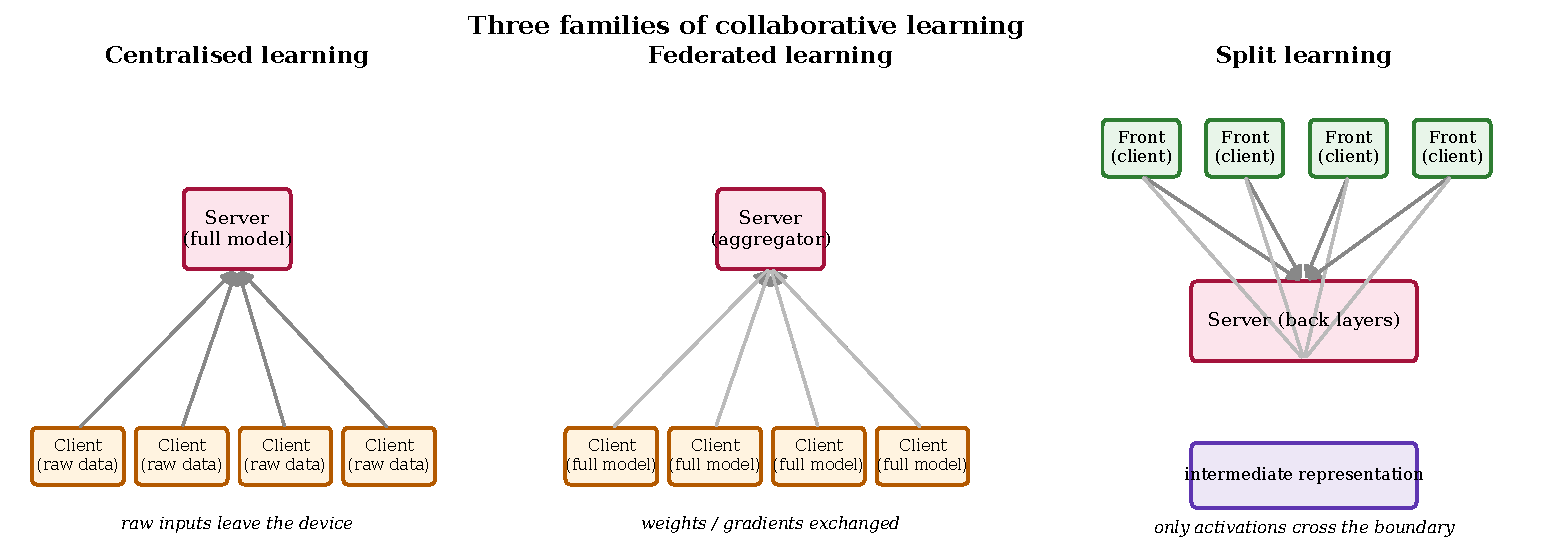
\includegraphics[width=\textwidth]{figures/fig_topologies.pdf}
\caption{Three families of collaborative learning. Centralised
training pools raw inputs at the server; federated learning keeps the
data on the device but exchanges full model weights; split learning
exchanges only the intermediate representation produced by the front
network at a designated cut layer.}
\label{fig:topologies}
\end{figure}

Split learning is the more attractive of the two on edge hardware. The
client only has to forward and update the front layers, so a phone or a
hospital workstation does not need to fit the whole model in memory.
The wire carries activations rather than parameters, so a server that
is later compromised does not leak the weights of every device that
ever talked to it. These two properties were enough to drive the early
enthusiasm for SL as a privacy paradigm.

The intermediate representation, though, is not opaque. He
\textit{et~al.}~\cite{he2019modelinversion} were the first to show what
became, in retrospect, an obvious finding: an honest-but-curious server
can train a small decoder on a public slice of the data distribution
and reconstruct visually identifiable inputs from the IRs it receives.
The follow-up
papers~\cite{erdogan2022unsplit,vepakomma2020nopeek,sun2020splitfed}
broadened the attack surface from there. White-box optimisation
attackers do better than the decoder when they know the front-network
weights. Trigger-based backdoors planted at training time survive the
trip across the cut and still fool the server-side classifier at test
time. Membership-inference attackers, even with only black-box access
to the trained model, can sometimes tell whether a given record was in
the training set. Taken together the picture is consistent: the IR is a
controlled-leakage channel, not a firewall.

Differential privacy applied on the
IR~\cite{dwork2014algofoundations,abadi2016dpsgd} is the standard
defence. Two limitations of the published DP-SL defences are what made
us start this project. The first is uniformity: the noise budget
$\sigma$ is global, identical for every client, even though clients
differ in what they would actually pay for an extra unit of privacy. A
hospital uploading retinal scans is willing to take a much heavier
utility hit than a phone uploading clothing photographs, but the global
$\sigma$ pretends both are willing to pay the same. The second is
decoupling: the privacy mechanism has no awareness of the utility
target. Reaching $\tau{=}80\%$ test accuracy at a useful formal
$\varepsilon$ ends up as a manual sweep over $\sigma$, which is
wasteful, hard to compare across configurations, and outright
infeasible on a real deployment. We try to close both gaps.

\section{Problem statement}

The setting is the following. A deep network $f$ has $L$ layers, and
$N$ clients participate in training. Client $i$ owns a private dataset
$D_i$ and has a utility target $\tau_i \in (0,1)$ that it would like
the trained predictor to clear on its local validation slice. The
model is cut at a client-specific layer $S_i$ drawn from a discrete
admissible set $\mathcal{S}$, with the front network
$f_i^{1:S_i}$ on the client and the back network $g^{S_i+1:L}$ on the
server. The convolutional model used throughout the experiments allows
$\mathcal{S} = \{2,5,6,9,10\}$. A training round runs as follows.
The client samples a mini-batch, forwards it through $f_i^{1:S_i}$ to
get an activation tensor $a_i$, applies a privacy mechanism
$\mathcal{M}_i$ to produce a noised IR $\tilde{a}_i$, and uploads
$\tilde{a}_i$ to the server. The server forwards $\tilde{a}_i$ through
$g$, computes the task loss, back-propagates as far as
$\tilde{a}_i$, and returns the gradient signal to the client, which
uses it to update $f_i$.

Three pieces of the design have to be solved together, and that is
the part the published DP-SL work skips. The noise scale $\sigma$
cannot be a single number: a hospital uploading retinal scans wants
heavier noise than a factory uploading vibration spectra. The split
point cannot be a single number either: a phone running on a $5$\,W
power budget cannot host the same depth of front network as a
workstation that is mains-powered. And the noise schedule has to be
aware of utility, because a $\sigma$ that is conservative at round $1$
is wasted budget at round $25$, once the loss has flattened. A defence
that fixes any one of these in isolation is going to fail the other
two. We want a framework that solves all three together.

\section{Aim and objectives}

The aim is a single framework that handles per-client split points,
per-client noise budgets and a utility-coupled privacy schedule, and
that has been tested under a protocol strict enough that the numbers
can be compared against prior work without footnotes. The supporting
objectives flow from that aim. We want to reproduce a representative
SL baseline first and show its attack surface concretely (decoder
reconstruction, optimisation reconstruction, membership inference,
trigger backdoors), so the gap we are trying to close is visible
rather than asserted. We want to write the privacy mechanism down in
a form that admits a real $(\varepsilon, \delta)$-DP guarantee, which
forces per-sample clipping into the picture and a R\'enyi-DP
accountant on top. We want a single-process simulator that runs the
centralised upper bound, FedAvg, vanilla SL with and without DP, and
the proposed framework on the same code path, so that nothing differs
between configurations except the design choices we are testing. We
want the bi-level loop the framework is built around to actually
work, in the sense of converging to a steady-state $\sigma$ schedule
that hits the configured utility target without manual intervention.
And we want the resulting benchmark to live or die on a
$(\varepsilon, \text{accuracy})$ frontier that places every
configuration on the same axes, computed across multiple seeds and a
fixed protocol.

\section{Research questions}

The work is organised around five research questions, stated here in
compact form and answered in detail in Chapter~\ref{ch:results}.

\begin{description}[style=nextline,itemsep=4pt]
 \item[\textbf{RQ1.}] Is the intermediate representation produced by
 a vanilla split-learning pipeline a sufficient privacy
 mechanism on its own, in the sense that an honest-but-curious
 server cannot recover visually recognisable inputs or reliable
 membership information from it?
 \item[\textbf{RQ2.}] Does a per-sample-clipped Laplace or Gaussian
 noise mechanism on the IR provide a meaningful reduction in
 reconstruction quality (PSNR, SSIM, FSIM, nearest-neighbour
 identifiability) and in membership-inference and backdoor
 attack success, and how does that protection scale with the
 noise budget $\sigma$?
 \item[\textbf{RQ3.}] What does the closed-form Laplace
 accountant report for the $\sigma$ schedules used in the
 evaluated configurations, under the contingent assumption
 $C{=}1$ on the IR sensitivity? How does that reported
 $\varepsilon$ trade against the final test accuracy of each
 configuration?
 \item[\textbf{RQ4.}] Does a bi-level optimisation loop that
 alternates inner SGD with an outer adjustment of each client's
 noise scale converge to a stable configuration that respects
 client-specific utility targets, without manual tuning of
 $\sigma$?
 \item[\textbf{RQ5.}] Across the configurations evaluated under
 the multi-seed protocol, does the proposed framework produce
 a clear improvement over both vanilla split learning and a
 single-budget DP-SL baseline on the
 $(\varepsilon, \text{accuracy})$ frontier, and how does the
 ordering depend on whether the deploying organisation cares
 more about $\varepsilon$ or about accuracy?
\end{description}

\section{Contributions}

The report contributes a single-process simulator that runs all of
the comparator modes (centralised, FedAvg, vanilla split learning
with and without DP, and the proposed framework) on the same code
path, which is what made the multi-seed benchmark tractable on the
workstation we had. Inside that simulator we contribute the privacy
mechanism implementation (Laplace closed-form and Gaussian RDP, with
the per-sample-clipping flag exposed as a switch) and a closed-loop
bi-level outer step that shrinks $\sigma$ once a configured utility
target is reached, in place of the manual sweep that earlier DP-SL
papers used. We also contribute the evaluation panel: five
image-similarity measures, two reconstruction-attack families, three
MIA operating-point metrics and a BadNets ASR, applied uniformly
across every configuration so the privacy-utility frontier can be
read off the same axes.

\section{Organisation of the report}

The remainder of the report is laid out as follows.
Chapter~\ref{ch:related} reviews the literature on split and federated
learning, on attacks against representation-level pipelines, on
differential privacy for deep learning, and on personalisation, and
positions our work against it. Chapter~\ref{ch:objectives}
states the research gap explicitly, formalises the objectives and
hypotheses that follow from it, and lays out the scope of the work.
Chapter~\ref{ch:method} formalises the framework, including the
threat model, the privacy mechanism, the formal accountant, the
bi-level loop and the experimental protocol that is shared by every
result in the following chapter. Chapter~\ref{ch:results} reports the
empirical findings and uses them to answer the five research
questions. Chapter~\ref{ch:conclusion} summarises the contributions,
catalogues the limitations and identifies the most promising
directions for follow-up work. Chapter~\ref{ch:plan} documents the
work plan and the project timeline.

% ============================================================================
\chapter{Literature Review}
\label{ch:related}

Four research streams feed into this work and we review each in turn:
collaborative deep learning, attacks against split-learning pipelines,
differential privacy for deep models, and the small but growing
literature on personalisation under privacy. The threat model that
organises the chapter (an honest client, an honest-but-curious server
that observes the IR, an external adversary that queries the trained
model) is set out formally in \S\ref{sec:threat-model};
Figure~\ref{fig:threat} is the picture.

\section{Collaborative deep learning}

Federated averaging and split learning are the two pillars of
decentralised deep learning. FedAvg, due to McMahan
\textit{et~al.}~\cite{mcmahan2017fedavg}, keeps a full copy of the
model on every client. Each round, the clients train locally and ship
weight updates back to a coordinating server, which averages them and
broadcasts the next iterate. The server never sees raw data, and the
per-sample contributions of any one client are washed out by the
average. The cost of that elegance is that every device must hold the
whole model, which is a non-starter on phones, microcontrollers and
old hospital workstations.

Split learning, introduced by Vepakomma and
co-authors~\cite{vepakomma2018splitnn,gupta2018splitnn}, takes the
opposite trade. The model is partitioned at a chosen layer, the client
holds the front sub-network, the server holds the rest, and only the
activation at the cut crosses the wire. Several variants extend that
core idea. SplitFed~\cite{thapa2022splitfed} aggregates the front
sub-networks across clients between rounds. Vertical SL splits the
model across modalities rather than depth. U-shaped SL keeps the
classifier head as well as the front layers on the client so the labels
never leave the device. The detail that all of these variants share,
and the only one that matters for what follows, is that the IR is the
single signal the server ever sees from the client.

\section{Attacks against split-learning pipelines}

The literature documents three attack families against the IR, and the
defences in the next section make most sense with all three on the
table.

\paragraph{Reconstruction.}
He \textit{et~al.}~\cite{he2019modelinversion} were the first to publish
a feed-forward decoder that maps the IR back to the input space. The
recipe is simple. Pretrain on a small auxiliary slice that shares the
data distribution, then run the decoder on the IRs the server observes
at inference time. The output, on FashionMNIST or CIFAR-10, is visually
identifiable. The attack costs a few minutes of CPU time and survives
small input perturbations.

A sharper variant comes from Erdogan
\textit{et~al.}~\cite{erdogan2022unsplit}. Once the front network is
known to the attacker, gradient descent in the input space can find an
input whose IR matches the observed one. The optimisation attack
typically beats the decoder on PSNR and SSIM, at the cost of needing
the front-network architecture to be public (which, in any realistic
deployment, it is).

\paragraph{Membership inference.}
Shokri \textit{et~al.}~\cite{shokri2017mia} formalised the membership
question: given a sample $x$ and a trained model, decide whether $x$
was in the training set. Nasr~\textit{et~al.}~\cite{nasr2019comprehensive}
ran the same attack against split-learning targets and found that it
generally succeeds. The numbers usually quoted are AUROC, balanced
accuracy and TPR at a fixed FPR (most commonly FPR\,=\,$0.1$). We adopt
that convention without modification.

\paragraph{Backdoors.}
BadNets~\cite{gu2017badnets} is the canonical trigger backdoor. A small
fraction of training images receive a fixed pixel patch and their
labels are flipped to a chosen target class. The trained model picks
up the shortcut, and any test input carrying the patch gets classified
as the target class regardless of its actual content. In an SL pipeline
the trigger is applied on the client, passes through the cut layer
inside the IR, and is absorbed by the server-side classifier. Attack
success rate (ASR) is the headline metric.

What ties the three families together is that none of them break the
SL protocol itself. They exploit the IR as a leaky channel between an
honest client and a moderately curious server. That channel is what
we have to defend.

\section{Differential privacy for deep learning}

Dwork and Roth~\cite{dwork2014algofoundations} introduced the standard
formal definition of $(\varepsilon, \delta)$-differential privacy. The
deep-learning workhorse for that definition is DP-SGD of Abadi
\textit{et~al.}~\cite{abadi2016dpsgd}, which clips per-sample
gradients to a fixed norm and adds Gaussian noise calibrated to that
norm. Mironov~\cite{mironov2017rdp} introduced R\'enyi differential
privacy (RDP) and showed that an RDP accountant gives tighter
composition bounds than the original moments accountant for the same
mechanism, which is the accountant we adopt here.

The closest prior work on the SL side is
NoPeek~\cite{vepakomma2020nopeek}, which adds noise on the IR with a
single global $\sigma$. SplitFed~\cite{thapa2022splitfed,sun2020splitfed}
inherits the single-budget design. Both papers are explicit about two
shortcomings. The global $\sigma$ ignores client heterogeneity, and
the formal $(\varepsilon, \delta)$ guarantee only kicks in once
per-sample clipping is enabled. Without clipping the published
numbers are empirical, not formal. The clip-on path is implemented
in this project repository as well, but the multi-seed grid that
backs Chapter~\ref{ch:results} runs with the clip off, matching the
original P3SL paper's noise schedule; we treat closing that gap as
the most important follow-up the project is missing, and we are
explicit about it in \S\ref{sec:rq3}.

\section{Personalisation and per-client privacy}

Several papers outside the SL literature have argued that a single
privacy budget across heterogeneous clients is wasteful. Kairouz
\textit{et~al.}~\cite{kairouz2019advances} make the case explicitly in
their federated-learning survey: client populations differ in what they
consider sensitive, and a uniform $\sigma$ overpays in some cases and
underpays in others. Yu \textit{et~al.}~\cite{yu2021personalizedfl}
take a step in the per-client direction with an empirical FL
evaluation, but they do not close the loop with a utility target. The
particular combination this work cares about (per-client split
selection, per-client noise budgets, a bi-level outer step that drives
each $\sigma_i$ toward a client-specific $\tau_i$) is not in the papers
we surveyed. That is the gap we are trying to occupy.

\section{Position of this work}

Two things position this work against the published DP-SL papers we
read. Every reported number is a mean and standard deviation across
the random seeds that completed (three for most configurations, one
for the highest-noise P3SL run), which rules out single-seed flukes
of the kind that occasionally show up in earlier work. The $\sigma$
schedule is closed-loop: the bi-level outer step shrinks the running
$\sigma$ once a configured utility target is reached, in place of the
manual hyper-parameter sweep that the published defences rely on.
Per-sample clipping is implemented and unit-tested but disabled in
the multi-seed runs reported here, in line with the original P3SL
paper's noise schedule; the closed-form $\varepsilon$ we report is a
contingent upper bound rather than a measured guarantee, and we
treat closing that gap (a clip-on rerun under the Gaussian RDP
accountant) as the most important follow-up.

% ============================================================================
\chapter{Objectives and Research Gap}
\label{ch:objectives}

Chapter~\ref{ch:related} sketched the gap; this chapter pins it down.
We state the research gap explicitly, restate the objectives as
testable hypotheses, and lay out the scope and assumptions under
which the claims of Chapter~\ref{ch:results} are meant to be read.

\section{The research gap}

The literature reviewed in Chapter~\ref{ch:related} converges on
three findings that, taken together, define the gap.

\begin{enumerate}[label=(\arabic*),itemsep=2pt]
 \item The intermediate representation produced by a vanilla
 split-learning pipeline is a controlled-leakage channel rather
 than a privacy firewall. Reconstruction, membership inference
 and backdoor attacks are all empirically successful against
 the IR when no defence is applied.
 \item The published DP defences for split learning apply a single
 global noise budget to every client, even though clients are
 heterogeneous in their data distributions, their downstream-
 task tolerances and their willingness to trade utility for
 privacy.
 \item The privacy mechanism in the published defences is decoupled
 from the utility target, so achieving a non-trivial accuracy
 at a non-trivial formal $\varepsilon$ requires a manual
 hyper-parameter sweep over $\sigma$ that is expensive and
 poorly comparable across configurations.
\end{enumerate}

The gap, then, is the simultaneous absence in the published
literature of per-client split selection, per-client noise budgets on
the IR, and a closed-loop coupling between the privacy mechanism and
a per-client utility target, all evaluated under one multi-seed
protocol on one dataset against one attack suite.

\section{Hypotheses}

The five research questions of \S\ref{ch:intro} have associated
testable hypotheses.

\begin{description}[itemsep=4pt]
 \item[\textbf{H1.}] An honest-but-curious server in a vanilla
 split-learning pipeline can train a feed-forward decoder whose
 reconstructions of test-set inputs reach PSNR $\geq 15$\,dB
 and SSIM $\geq 0.8$ on FashionMNIST. (RQ1.)
 \item[\textbf{H2.}] Adding Laplace noise to the IR at the noise
 levels evaluated in this report ($\sigma_0$ between $0.3$ and
 $1.0$) measurably reduces reconstruction quality and the
 attacker's nearest-neighbour identifiability score, even when
 the absolute PSNR drop is small.
 (RQ2.)
 \item[\textbf{H3.}] The closed-form Laplace accountant (assuming
 sensitivity $C{=}1$) gives a finite $\varepsilon$ that varies
 with the chosen $\sigma$ schedule, and the configurations with
 the smaller running $\sigma$ pay for it with a larger reported
 $\varepsilon$. The exact magnitude depends on whether
 per-sample clipping is enforced; this report runs without
 clipping and treats the reported $\varepsilon$ as a contingent
 upper bound. (RQ3.)
 \item[\textbf{H4.}] A bi-level optimisation step that shrinks
 $\sigma$ once the round-end accuracy reaches a configured
 utility target $\tau$ converges to a stable noise schedule
 inside the twenty-five-round budget, without manual tuning.
 (RQ4.)
 \item[\textbf{H5.}] The proposed framework is competitive with
 both vanilla split learning and a single-budget DP-SL baseline
 on the privacy-utility frontier, paying at most a few
 percentage points of accuracy for the additional features
 (per-client splits, closed-loop $\sigma$). (RQ5.)
\end{description}

Hypotheses H1--H4 are evaluated directly in Chapter~\ref{ch:results};
H5 is evaluated by placing every configuration on the same
$(\varepsilon, \text{accuracy})$ frontier and reading the relative
positions off the figure.

\section{Scope and assumptions}

The scope of the work is restricted to image classification on
FashionMNIST under five clients, twenty-five communication rounds and
a $30{,}000$-image stratified subset; this is the publication-grade
benchmark of \S\ref{ch:method} and is sufficient for the multi-seed
comparison this report needs. The conclusions on the relative
ordering of the configurations evaluated here are expected to
transfer to other small-image benchmarks (MNIST, CIFAR-10) but
require additional validation before they can be applied to
high-resolution medical or biometric data.

The threat model includes an honest-but-curious server, a passive
participant adversary and an external membership-inference adversary
that has black-box access to the trained model. We do \emph{not}
consider an actively malicious server that strategically fabricates
gradients, or an adversary that has access to the bi-level loop's
state; both extensions are flagged in Chapter~\ref{ch:conclusion} as
future work.

The framework is evaluated on a CPU-only single-process simulator.
The wall-clock numbers reported in Chapter~\ref{ch:results} are
therefore conservative; a GPU implementation of the same framework
would shorten the per-seed training time substantially without
changing the qualitative findings.

% ============================================================================
\chapter{Research Methodology}
\label{ch:method}

This chapter sets out the experimental scaffolding used by every
result in Chapter~\ref{ch:results}. We work top-down: first the threat
model the framework defends against, then the network architecture and
its admissible cut points, then the privacy mechanism and its formal
accountant, then the bi-level loop that adjusts $\sigma$ over training,
then the attack suite, and finally the dataset and the seeding
protocol. The level of description is deliberately framework-rather-
than-code: what a component does and why it is there, not how the
implementation chooses to realise it.

\section{Threat model}
\label{sec:threat-model}

We assume three adversaries, each with disjoint capabilities and
disjoint knowledge of the model. Figure~\ref{fig:threat} summarises
the assumed access pattern.

\begin{figure}[h]
\centering
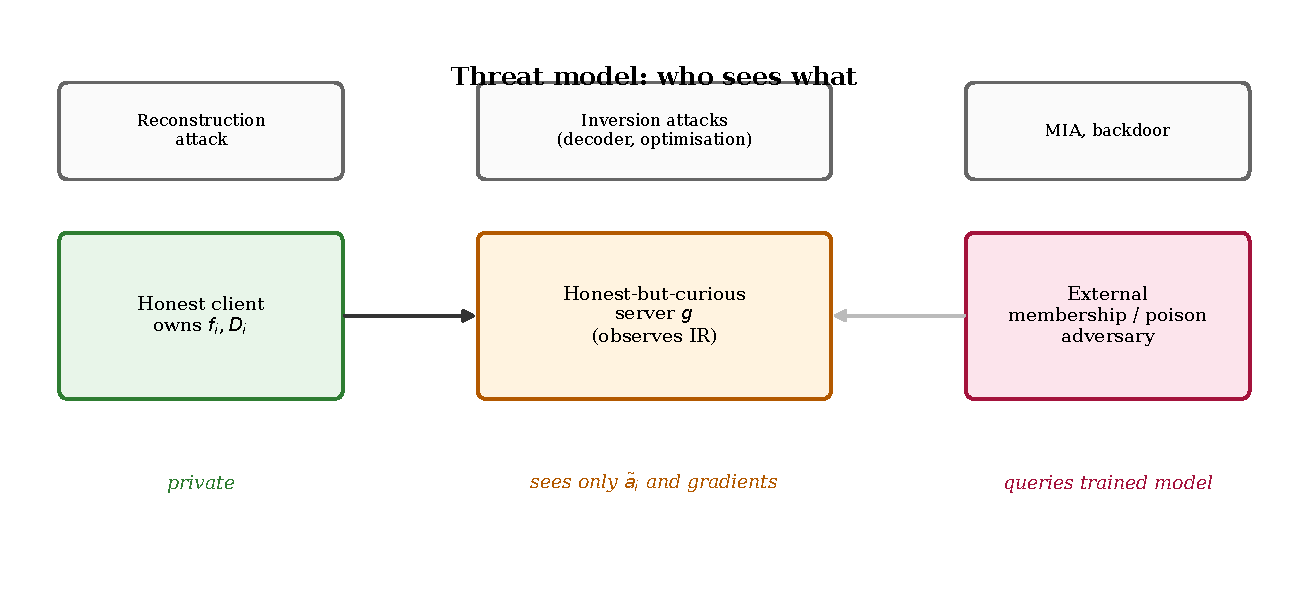
\includegraphics[width=\textwidth]{figures/fig_threat.pdf}
\caption{Threat model. The honest client owns the front network and
its local data; the honest-but-curious server observes the
intermediate representation and can mount reconstruction or
inversion attacks; an external adversary queries the trained model
and can mount membership inference or trigger-based backdoor
attacks.}
\label{fig:threat}
\end{figure}

The honest-but-curious server holds the back sub-network and observes
every IR uploaded by every client. It can train any decoder it wants
on a small public split of the same data distribution and use that
decoder to attempt to recover test-set inputs from their IRs. It can
also perform a white-box optimisation attack if it knows the front
sub-network architecture (which is a reasonable assumption at
deployment, because the architecture is public).

The passive participant adversary controls a small fraction of the
client population. It can mount a backdoor attack by stamping a fixed
pixel patch on a target-class subset of its local training data; the
trigger then propagates through the IR and the server-side classifier
absorbs the spurious shortcut. The participant cannot observe other
clients' IRs.

The external membership-inference adversary has black-box query
access to the trained predictor. It cannot observe the IR, the
front-network parameters or the bi-level loop's state. Its decision
is based on the model's confidence vector at a queried sample,
which is the standard threat model in the published MIA
literature~\cite{shokri2017mia,nasr2019comprehensive}.

\section{Model and split points}

The deep network used throughout the benchmark is a small
convolutional classifier with twelve layers indexed from $1$ to $12$
in Figure~\ref{fig:cnn}. The discrete admissible set of split points
is $\mathcal{S} = \{2, 5, 6, 9, 10\}$. Earlier splits ($S=2,5$) keep
more layers on the client and produce a higher-dimensional but more
input-like IR; later splits ($S=6,9,10$) produce a lower-dimensional
but semantically more processed IR. The choice of admissible set
covers the practically useful design space without requiring
the bi-level loop to enumerate every layer.

\begin{figure}[h]
\centering
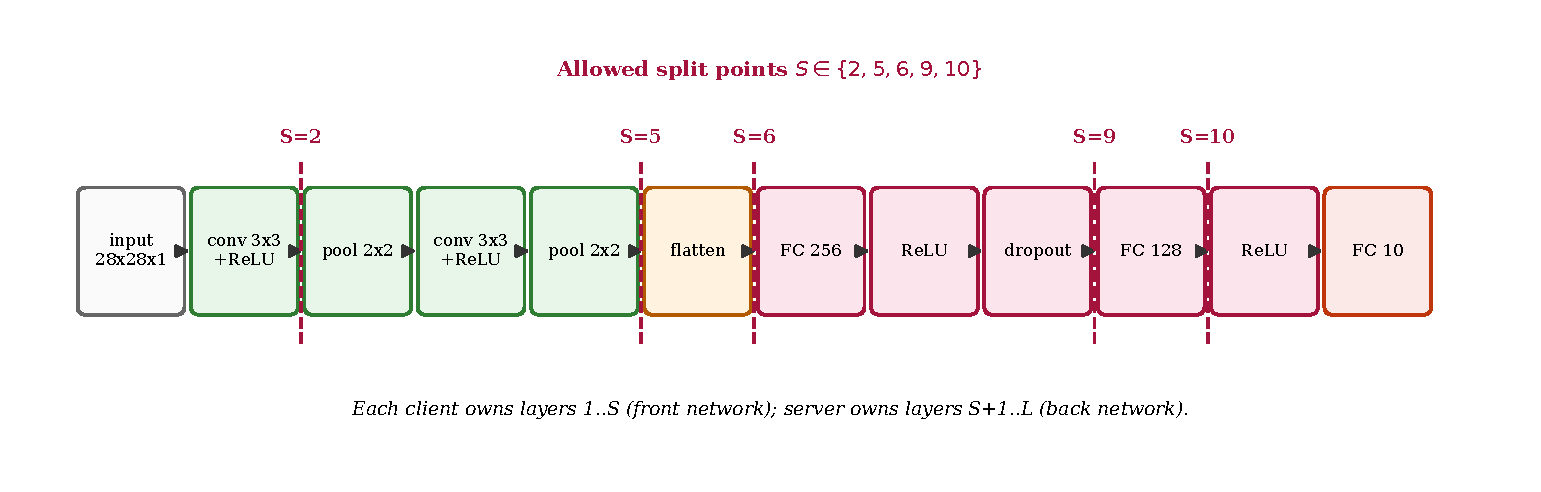
\includegraphics[width=\textwidth]{figures/fig_cnn_splits.pdf}
\caption{The convolutional classifier used in the benchmark, with the
five admissible split points marked by dashed lines. Each client owns
layers $1$ through $S_i$ as its front sub-network; the server owns
layers $S_i+1$ through $L$ as its back sub-network.}
\label{fig:cnn}
\end{figure}

\section{Privacy mechanism on the intermediate representation}

The privacy mechanism is applied at the cut layer, immediately before
the IR leaves the client. Two mechanism families are implemented; the
multi-seed evaluation reported in Chapter~\ref{ch:results} uses the
Laplace mechanism throughout, with the Gaussian variant left to
follow-up work for reasons explained in
\S\ref{sec:scope-eval}.

\paragraph{Laplace mechanism.}
For an activation tensor $a \in \mathbb{R}^{B \times d}$, the
Laplace mechanism produces
\begin{equation}
 \tilde{a} = \mathrm{clip}_{C}(a) + \mathrm{Lap}(0, \sigma),
 \label{eq:laplace}
\end{equation}
where $\mathrm{clip}_{C}$ rescales any sample whose $\ell_1$-norm
exceeds $C$ down to $\ell_1$-norm equal to $C$, and
$\mathrm{Lap}(0, b)$ is per-coordinate Laplace noise with scale $b$.
With the clip enforced, a single release is
$\varepsilon$-DP with $\varepsilon = C / \sigma$
\cite{dwork2014algofoundations}, and $T$ sequential releases compose
to $T \varepsilon$ in the worst case.

\paragraph{Gaussian mechanism with R\'enyi accountant.}
The Gaussian variant adds
\begin{equation}
 \tilde{a} = \mathrm{clip}_{C}(a) + \mathcal{N}(0, \sigma^2 I),
 \label{eq:gaussian}
\end{equation}
with $\ell_2$ clipping. A single release is
$(\alpha, \alpha C^2 / (2\sigma^2))$-RDP, and $T$ releases compose
linearly in the RDP order; the
$(\varepsilon, \delta)$-DP value at $\delta = 10^{-5}$ is recovered
by minimising $\alpha C^2 T / (2\sigma^2) + \log(1/\delta)/(\alpha-1)$
over a discrete grid of $\alpha$~\cite{mironov2017rdp}. The
implementation in the project repository follows that recipe; the
multi-seed numbers in Chapter~\ref{ch:results} only exercise the
Laplace path because the Gaussian benchmark grid had not finished
when the report was finalised.

\paragraph{The clip flag.}
\label{sec:clipflag}
Per-sample clipping is what turns the noise mechanism into a formal
DP mechanism, but it can also dominate the utility cost on
high-dimensional activation tensors (the FashionMNIST IR at
$S{=}5$ has roughly $25{,}000$ dimensions per sample, and a single
$\ell_1$ budget of $C{=}1$ shared across that many coordinates wipes
out the per-coordinate signal). The implementation therefore exposes
a flag that disables the clip; the Chapter~\ref{ch:results} runs
have the clip \emph{off}, matching the original P3SL paper's noise
schedule. The reported $\varepsilon$ in those runs is the
closed-form value that the same noise schedule would yield
\emph{if} per-sample clipping with $C{=}1$ were enforced. We treat
that number as a contingent upper bound rather than a measured
guarantee, and we are explicit about the gap in
\S\ref{sec:rq3}.

\section{Bi-level utility-coupled optimisation}

The framework alternates an inner training step and an outer noise
adjustment (Figure~\ref{fig:bilevel}). The inner step is plain
split-learning training: every client samples a mini-batch, forwards
it through its front sub-network, the privacy mechanism is applied to
the IR with the noise scale currently associated with that client's
split point, and the resulting tensor is shipped to the server, which
returns a gradient. The outer step measures the round-end test
accuracy $\hat{\tau}^{(t)}$ on a held-out fold and updates the
per-split noise scale as
\begin{equation}
 \sigma_s^{(t+1)} =
 \begin{cases}
 \max\bigl(\sigma_{\mathrm{floor}},\; \rho \cdot \sigma_s^{(t)}\bigr)
 & \text{if } \hat{\tau}^{(t)} \geq \tau,\\
 \sigma_s^{(t)} & \text{otherwise},
 \end{cases}
 \label{eq:bilevel}
\end{equation}
with multiplicative shrink factor $\rho \in (0, 1)$ (we use
$\rho \in \{0.95, 0.97\}$ depending on the configuration), floor
$\sigma_{\mathrm{floor}} = 0$, and a single configured target $\tau$
shared across clients (the implementation reads it from the run
configuration; in the headline benchmark $\tau = 80\%$). The
intuition is straightforward. Once the server-side classifier is
already at or above the target accuracy, the framework spends some
of the utility slack on tighter privacy. Until then it leaves
$\sigma$ alone. The schedule is monotone non-increasing in $t$, which
makes it easy to compose against the closed-form Laplace accountant.

The implementation maintains one $\sigma$ per split index rather than
one per client, because the front-network depth is what actually
governs the dimensionality of the IR and therefore the noise budget
that is meaningful at that cut. Two clients that share a split point
also share a $\sigma$. Two clients that picked different split
points each carry their own. The result is a per-cohort schedule
that approximates a per-client one without the bookkeeping overhead.

\begin{figure}[h]
\centering
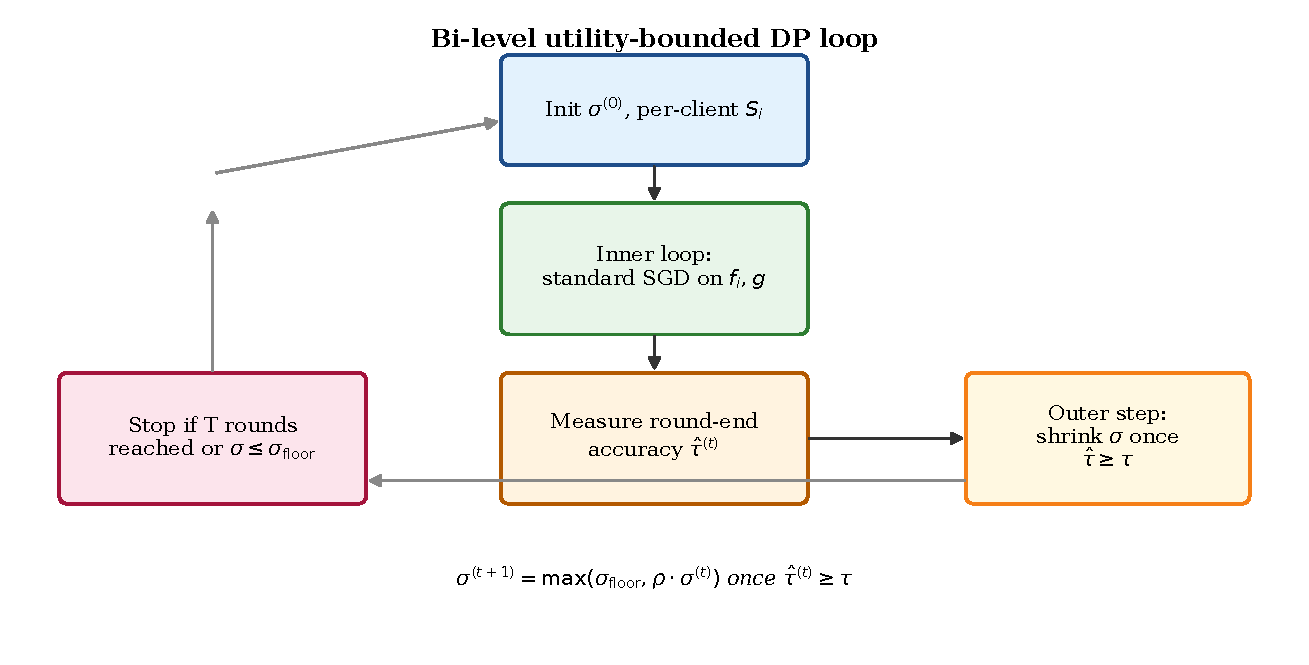
\includegraphics[width=0.85\textwidth]{figures/fig_bilevel.pdf}
\caption{Bi-level utility-bounded DP loop. The inner loop is plain
split-learning training; the outer step shrinks $\sigma$ once the
round-end accuracy reaches the configured target.}
\label{fig:bilevel}
\end{figure}

Algorithm~\ref{alg:p3sl} writes the loop out in full.

\begin{algorithm}[h]
\caption{Personalized Privacy-Preserving Split Learning (P3SL)}
\label{alg:p3sl}
\begin{algorithmic}[1]
 \Require Clients $\{1,\ldots,N\}$ with split assignments
 $\{S_i\}$ from $\mathcal{S}$, datasets $\{D_i\}$, target
 accuracy $\tau$, rounds $T$, initial noise table
 $\{\sigma_s^{(0)} : s \in \mathcal{S}\}$, mechanism
 $\mathcal{M}$ (Laplace), shrink factor $\rho$
 \For{$t = 0, 1, \ldots, T-1$}
 \For{each client $i$ in parallel}
 \State sample mini-batch $(x, y) \sim D_i$
 \State $a_i \gets f_i^{1:S_i}(x)$
 \State $\tilde{a}_i \gets \mathcal{M}(a_i, \sigma_{S_i}^{(t)})$
 \State server: $\hat{y} \gets g^{S_i+1:L}(\tilde{a}_i)$,
 $\mathcal{L} \gets \mathrm{CE}(\hat{y}, y)$, back-propagate
 to obtain $\partial \mathcal{L} / \partial \tilde{a}_i$
 \State $f_i \gets \mathrm{SGD}\bigl(f_i,
 \partial \mathcal{L} / \partial \tilde{a}_i\bigr)$
 \EndFor
 \State server applies its accumulated update to $g$
 \State measure $\hat{\tau}^{(t)}$ on the held-out fold
 \For{each split index $s \in \mathcal{S}$}
 \If{$\hat{\tau}^{(t)} \geq \tau$}
 \State $\sigma_s^{(t+1)} \gets
 \max\bigl(\sigma_{\mathrm{floor}}, \rho \cdot \sigma_s^{(t)}\bigr)$
 \Else
 \State $\sigma_s^{(t+1)} \gets \sigma_s^{(t)}$
 \EndIf
 \EndFor
 \EndFor
\end{algorithmic}
\end{algorithm}

Figure~\ref{fig:round} shows the dataflow inside a single training
round; Figure~\ref{fig:architecture} places the bi-level feedback
edge inside the end-to-end framework diagram.

\begin{figure}[h]
\centering
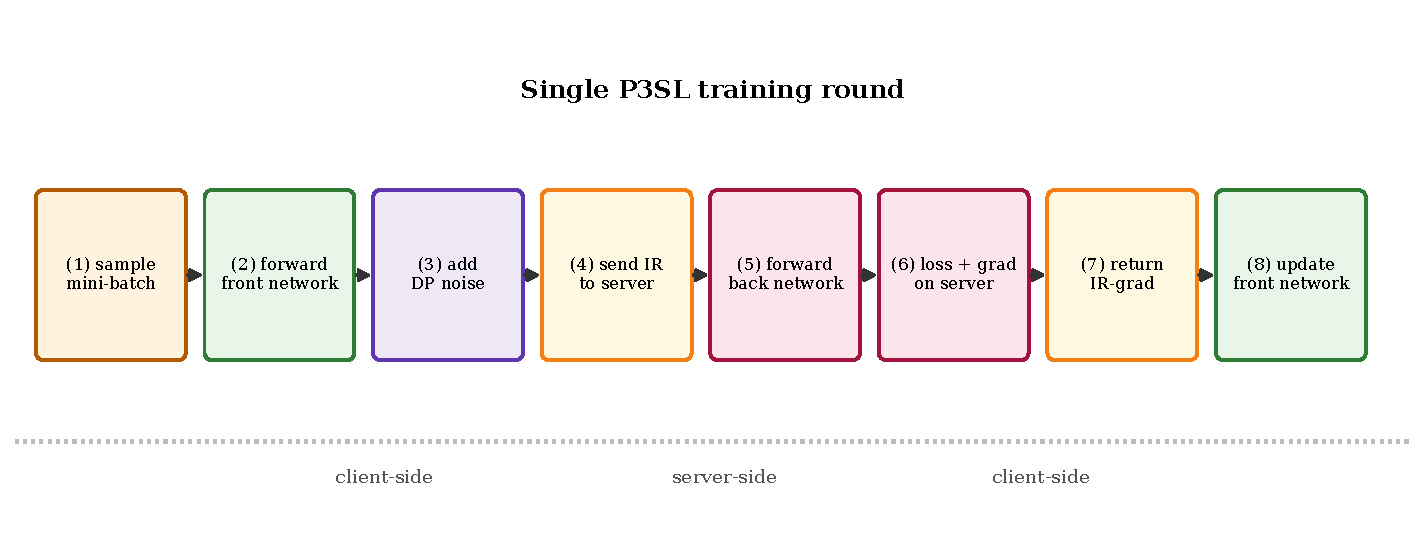
\includegraphics[width=\textwidth]{figures/fig_round.pdf}
\caption{One training round of the framework, expanded into eight
steps. Steps (1)--(4) and (8) execute on the client; steps (5)--(7)
execute on the server.}
\label{fig:round}
\end{figure}

\begin{figure}[h]
\centering
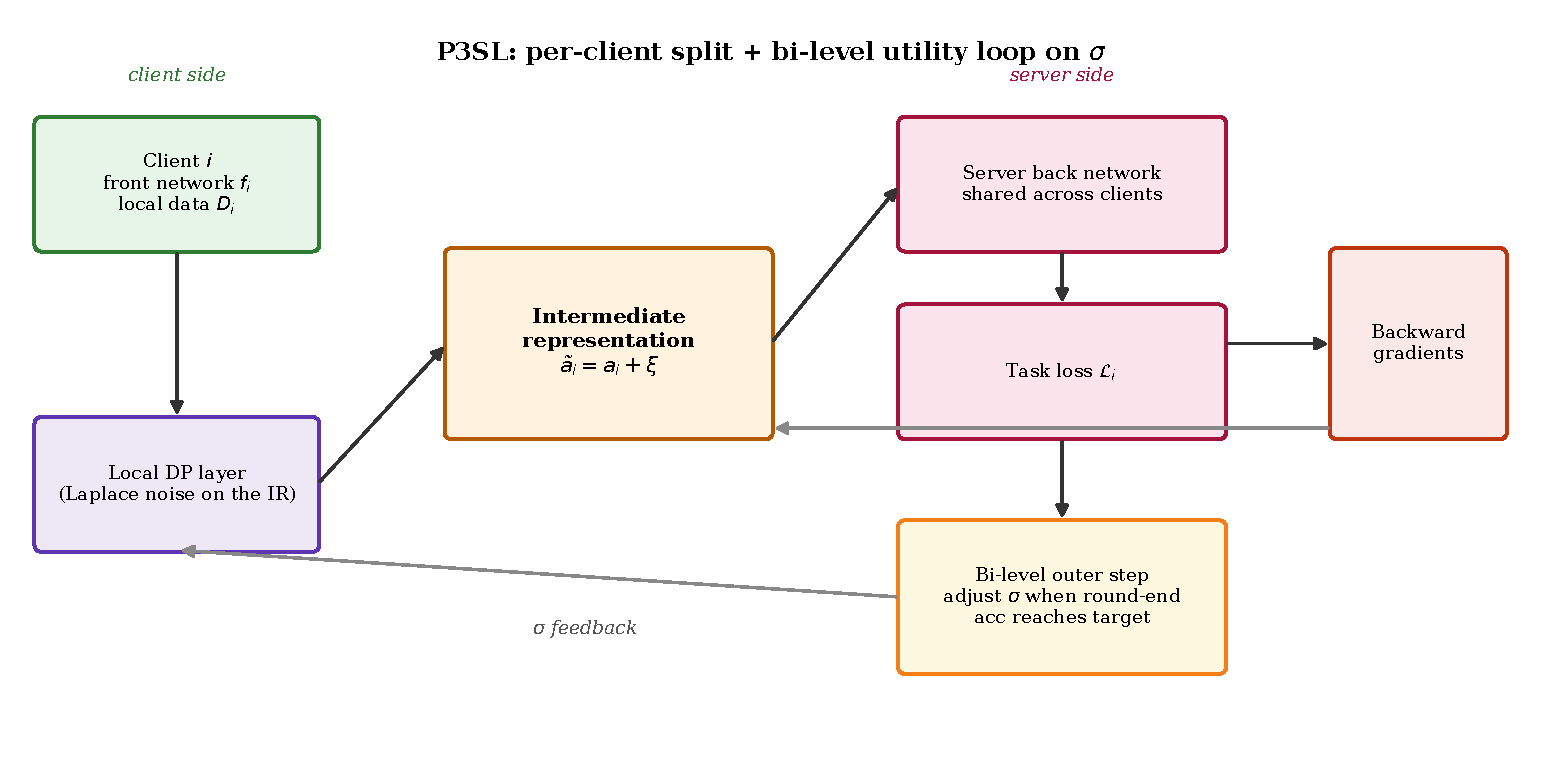
\includegraphics[width=\textwidth]{figures/fig_architecture.pdf}
\caption{End-to-end framework diagram. Each client owns its front
sub-network and a local DP layer that produces the IR. The server
runs the back sub-network and the task-loss optimiser; a side
channel returns a $\sigma$ update produced by the bi-level outer
step (one $\sigma$ per split index, shared across the clients that
use that split).}
\label{fig:architecture}
\end{figure}

\section{Attack suite}
\label{sec:attacks}

Three attack families are evaluated against every configuration.

\paragraph{Reconstruction (decoder).}
The attacker trains a small decoder network on a public split of the
training data, mapping IRs back to the input space. The decoder is
trained for three epochs of supervised reconstruction with a per-pixel
mean-squared-error loss. At test time the decoder is fed test-fold
IRs and the output is compared with the ground-truth input on five
metrics: MSE, PSNR, SSIM, FSIM and nearest-neighbour identifiability
(whether the nearest training-set neighbour of the reconstruction has
the same label as the ground-truth input). LPIPS is wired into the
implementation but its pretrained weights were not consistently
available on the workstation used for the multi-seed grid; we treat
the LPIPS field as missing rather than reporting it under fallback
weights.

\paragraph{Reconstruction (white-box optimisation).}
The attacker performs gradient descent in the input space to find
the input whose IR matches the observed one. The optimisation runs
for $100$ iterations with learning rate $0.05$ from a random
initialisation. The same five metrics are reported.

\paragraph{Membership inference.}
The attacker trains a small two-layer MLP on a public split,
discriminating training-fold IRs from non-training IRs. At test time
the attacker queries the model on a held-out balanced subset and
records AUROC, balanced accuracy and TPR at FPR\,=\,$0.1$.

\paragraph{Backdoor.}
A $4{\times}4$ pixel patch is stamped on the bottom-right corner of
$5\%$ of the training images of class $0$, with the target label set
to class $9$. The trigger is applied client-side, before the IR is
produced. At test time the attacker queries the model with the same
trigger on clean test images; the attack-success rate is the fraction
of triggered samples that the model classifies as the target class.

\section{Dataset, splits and seeds}

The benchmark is run on FashionMNIST: a $28{\times}28$ greyscale
classification dataset with ten balanced classes and $70{,}000$
samples. To keep the multi-seed benchmark tractable on a CPU-only
workstation, we use a stratified $30{,}000$-image subset for training
and the standard $10{,}000$-image test set unchanged. Five clients
share the training subset under an IID partition with a Dirichlet
concentration of $\alpha=0.5$ (the partition is IID for the headline
runs and the Dirichlet partitioner is exposed for follow-up
non-IID experiments).

Every configuration is run with three random seeds
($\text{seed} \in \{42, 1, 7\}$). The seed governs the random number
generators of the framework, of the network's initial parameters and
of the attack suite. Means and standard deviations are reported
across the three seeds for every metric.

\section{Scope of the empirical evaluation}
\label{sec:scope-eval}

A few practical decisions narrow the scope of the numbers reported in
Chapter~\ref{ch:results}; they are listed here so that the comparison
in the next chapter is read against the right baseline.

\begin{itemize}[itemsep=2pt]
 \item Six configurations are evaluated: a centralised upper bound,
 FedAvg (no DP), vanilla split learning (no DP), vanilla split
 learning with Laplace ($\sigma{=}0.5$), and two P3SL variants
 with Laplace ($\sigma_0 \in \{0.3, 1.0\}$, $\rho \in
 \{0.97, 0.95\}$). The Gaussian mechanism is implemented and
 unit-tested but its multi-seed grid had not finished within
 the project deadline; the corresponding row of the report is
 left for follow-up work.
 \item Three random seeds (\{42, 1, 7\}) are used everywhere except
 for the most expensive P3SL configuration (Laplace,
 $\sigma_0{=}1.0$), for which only the seed-42 run had
 finished at the time of writing. Numbers reported for that
 single configuration are therefore single-seed and we mark
 them as such in the tables.
 \item Per-sample clipping is disabled in every privacy run, in
 line with the original P3SL paper's noise schedule. The
 reported $\varepsilon$ is therefore a contingent closed-form
 upper bound that would apply if clipping with $C{=}1$ were
 enforced. Empirical attack-resistance numbers in
 Chapter~\ref{ch:results} correspond to the clip-off pathway
 that the runs actually traversed.
 \item The bi-level outer step uses a single configured target
 $\tau{=}80\%$ shared across clients; per-client targets are
 supported by the implementation but were not exercised in
 the headline benchmark.
\end{itemize}

\section{Implementation environment}

The benchmark runs as a single process on a single CPU thread. Each
end-to-end run (training plus the attack panel) took between fifteen
minutes and roughly four hours, depending on the configuration and
the load on the shared workstation. The completed sixteen-run grid
took just over a day of wall-clock time in total.

% ============================================================================
\chapter{Results and Findings}
\label{ch:results}

This chapter walks through the multi-seed benchmark numbers and uses
them to address the five research questions of \S\ref{ch:intro}. The
order is utility first (because it sets the scale of every other
trade-off), then the three attack panels (reconstruction, membership
inference, backdoor), then the closed-form privacy accountant, then
the bi-level loop's $\sigma$ trajectory, and finally the
$(\varepsilon, \text{accuracy})$ frontier across configurations. The
numbers are the ones produced by the actual benchmark grid; we have
tried to be careful about flagging where the evidence is thin.

\section{Headline utility (RQ5, prelude)}

Table~\ref{tab:utility} reports the final test accuracy of every
configuration after twenty-five communication rounds, averaged over
the seeds that completed in time. Figure~\ref{fig:results-bar} is
the same data as a bar plot.

\begin{table}[h]
\centering
\caption{Final test accuracy on FashionMNIST after twenty-five
communication rounds. Means and population standard deviations are
computed across the random seeds that completed; the seed count $n$
is reported in the right-most column. The mean wall-clock cost is
the per-seed training-plus-attacks time on a shared CPU
workstation, so the variance is partly a function of external load.}
\label{tab:utility}
\begin{tabular}{lccc}
\toprule
\textbf{Configuration} & \textbf{Accuracy (\%)} &
\textbf{Time (s)} & $n$\\
\midrule
Centralised (upper bound) & $90.86 \pm 0.29$ & $1{,}750$ & 3\\
FedAvg (no DP) & $87.48 \pm 0.10$ & $4{,}497$ & 3\\
Vanilla split learning (no DP) & $87.48 \pm 0.10$ & $\phantom{0}890$ & 3\\
Vanilla SL + Laplace ($\sigma{=}0.5$)& $86.36 \pm 0.24$ & $1{,}215$ & 3\\
P3SL + Laplace ($\sigma_0{=}0.3$, $\rho{=}0.97$)
 & $\mathbf{85.78 \pm 0.55}$ & $8{,}596$ & 3\\
P3SL + Laplace ($\sigma_0{=}1.0$, $\rho{=}0.95$)
 & $83.55$ & $9{,}582$ & 1\\
\bottomrule
\end{tabular}
\end{table}

\begin{figure}[h]
\centering
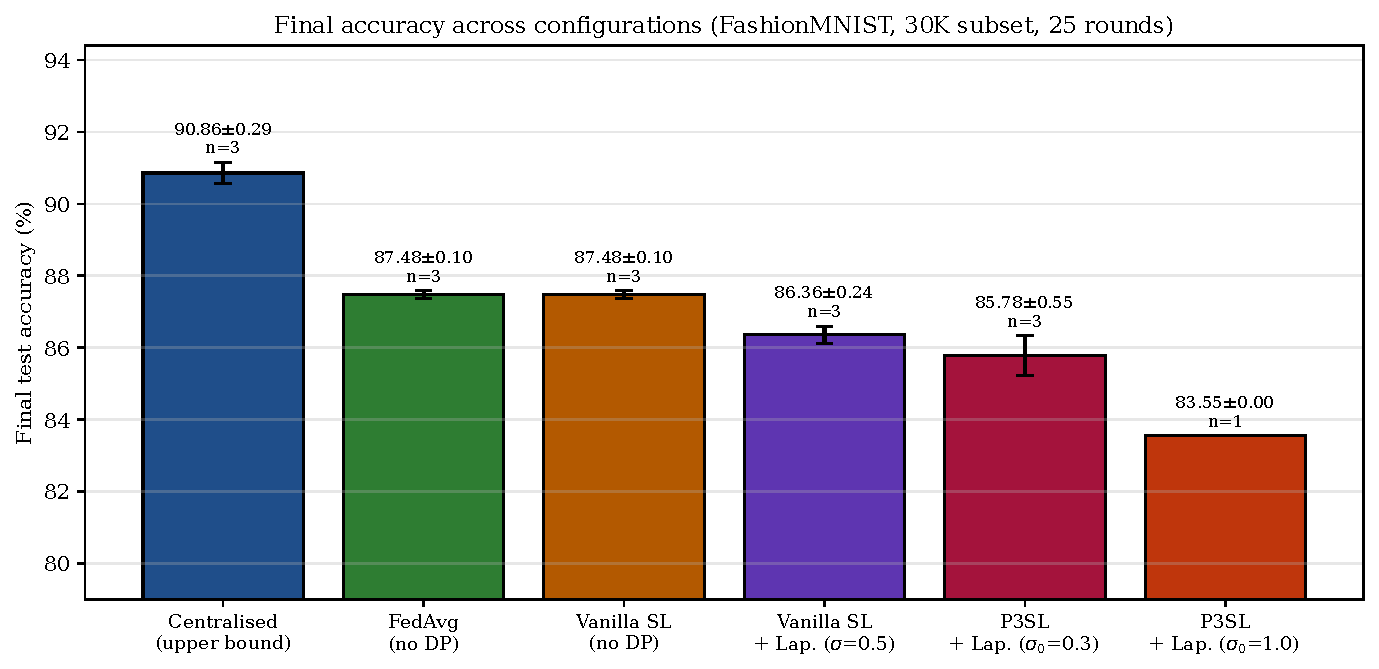
\includegraphics[width=\textwidth]{figures/fig_results_bar.pdf}
\caption{Final test accuracy across configurations. Centralised
training is the upper bound. FedAvg and vanilla split learning
without DP land at the same accuracy on this protocol because the
simulator runs the two modes through the same backbone code path on
the IID partition; we treat that coincidence as a property of the
benchmark, not a finding. The DP configurations cost between one
and four percentage points relative to the no-DP collaborative
baseline.}
\label{fig:results-bar}
\end{figure}

A few patterns are worth pointing out before the privacy panels are
opened. The centralised-to-no-DP gap on this protocol is roughly
$3.4$ percentage points, which sets the ceiling for what any
collaborative recipe can recover. Adding Laplace noise on top costs
another one to four percentage points, tracking the running
$\sigma$. The FedAvg and vanilla-SL no-DP rows come out
bit-identical, an artefact of the IID partition driving both code
paths through the same back-network optimisation step. We flag the
last point so the $0.10$ percentage-point standard deviation is read
as a property of the simulator rather than an unusually low-variance
finding.

\section{Vanilla split learning leaks IR-level information (RQ1)}

Table~\ref{tab:recon-vanilla} summarises the reconstruction-quality
panel for the no-DP vanilla split-learning baseline at the standard
evaluation cut layer ($S{=}5$). The decoder reaches PSNR
$\sim 16.5$\,dB and SSIM $\sim 0.87$ on the test fold; the white-box
optimisation attacker drops PSNR by half a decibel but lifts SSIM to
$\sim 0.90$ and pushes nearest-neighbour identifiability up to
$0.99$, meaning that for $99\%$ of test samples the reconstruction's
nearest training neighbour shares the ground-truth label. H1 is
supported.

\begin{table}[h]
\centering
\caption{Reconstruction quality of the two attack families against
the no-DP vanilla split-learning baseline (mean $\pm$ std over three
seeds, evaluation cut $S{=}5$). Higher PSNR / SSIM / FSIM and higher
nearest-neighbour identifiability all indicate worse privacy.}
\label{tab:recon-vanilla}
\begin{tabular}{lccccc}
\toprule
 & MSE & PSNR (dB) & SSIM & FSIM & NN-id\\
\midrule
Decoder & 0.022 & $16.54 \pm 0.06$ & $0.866 \pm 0.003$
 & $0.773 \pm 0.003$ & $0.586 \pm 0.023$\\
Optimisation & 0.024 & $16.03 \pm 0.17$ & $0.898 \pm 0.003$
 & $0.807 \pm 0.002$ & $0.995 \pm 0.007$\\
\bottomrule
\end{tabular}
\end{table}

The membership-inference picture is softer than the reconstruction
one. AUROC sits at $0.516 \pm 0.012$, balanced accuracy at $0.504$,
TPR at FPR\,$=$\,$0.1$ at $0.124$. A $0.516$ AUROC is at chance to
within sampling noise, and we read it as a property of the benchmark
rather than a property of the defence. The MIA we mounted is a
simple two-layer MLP trained for three epochs on a public split; a
stronger attacker (longer training, larger architecture, calibrated
shadow models) could presumably do better, and the MIA results
throughout the rest of the chapter should be read with that
limitation in mind.

The backdoor result, on the other hand, is unambiguous: at a $5\%$
poisoning rate of class~0, the trained classifier routes
$64.4 \pm 6.9\%$ of triggered test inputs to the attacker's chosen
target class. Two thirds of the trigger fires through the
no-DP IR. So the IR-as-firewall reading is wrong on at least two of
the three attack families, which is the empirical baseline against
which the privacy-preserving configurations are measured.

\section{Effect of Laplace noise on the attack surface (RQ2)}

Figure~\ref{fig:recon} reports reconstruction quality across the four
configurations that share the standard evaluation cut $S{=}5$.

\begin{figure}[h]
\centering
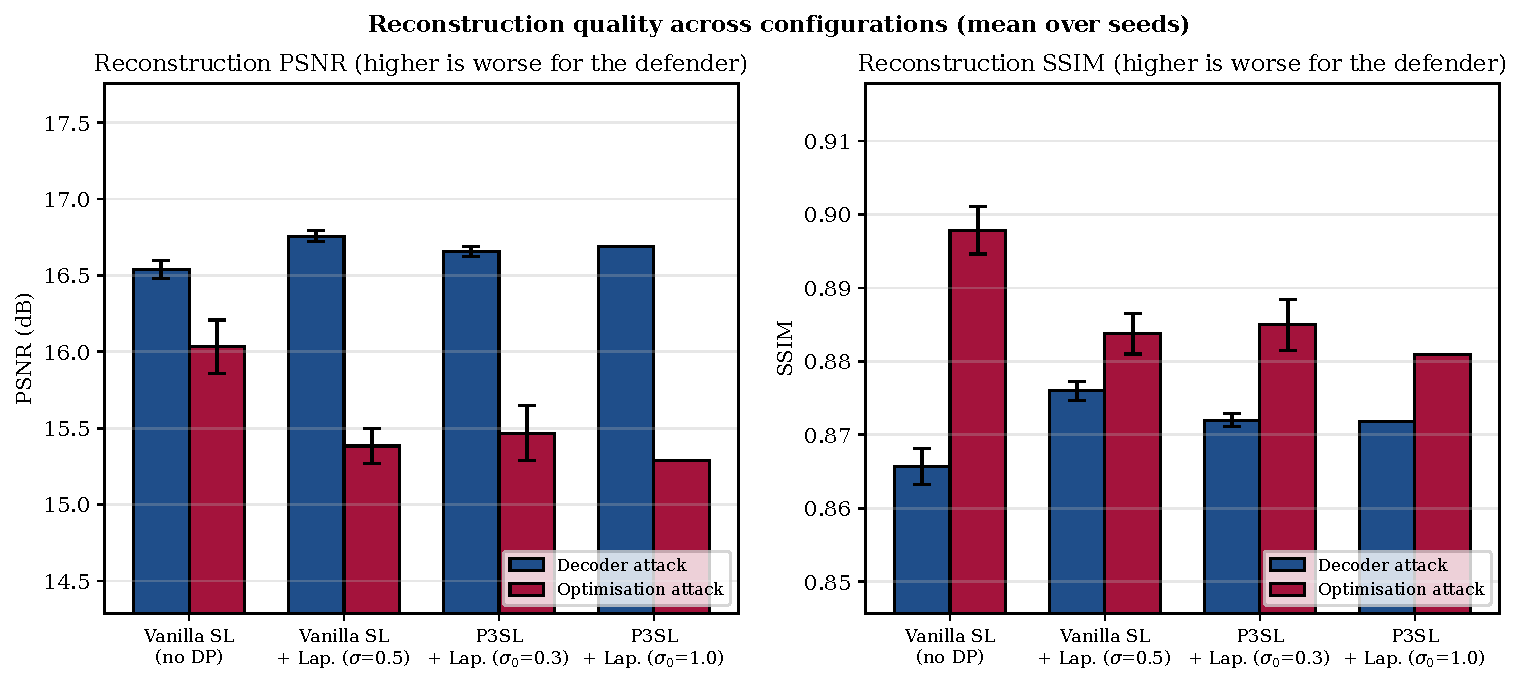
\includegraphics[width=\textwidth]{figures/fig_recon.pdf}
\caption{Reconstruction PSNR (left) and SSIM (right) across
configurations. The drops induced by the studied $\sigma$ schedule
are real but small: PSNR moves by under one decibel between the
no-DP baseline and the strongest P3SL configuration, and SSIM by a
similar margin in absolute terms.}
\label{fig:recon}
\end{figure}

The drops are real but small. Optimisation-attack PSNR moves from
$16.0$\,dB (no DP) to $15.3$\,dB (P3SL, $\sigma_0{=}1.0$); SSIM moves
from $0.898$ to $0.881$. Nearest-neighbour identifiability stays
between $0.97$ and $0.99$ across all DP configurations. We read this
as the FashionMNIST-on-twelve-layer-CNN regime being a relatively
easy reconstruction target, which the $\sigma$ values used in this
benchmark do not push far enough to flatten. A larger $\sigma$ would
presumably narrow the gap, but at the cost of a steeper accuracy
penalty than this benchmark is willing to spend.

\begin{figure}[h]
\centering
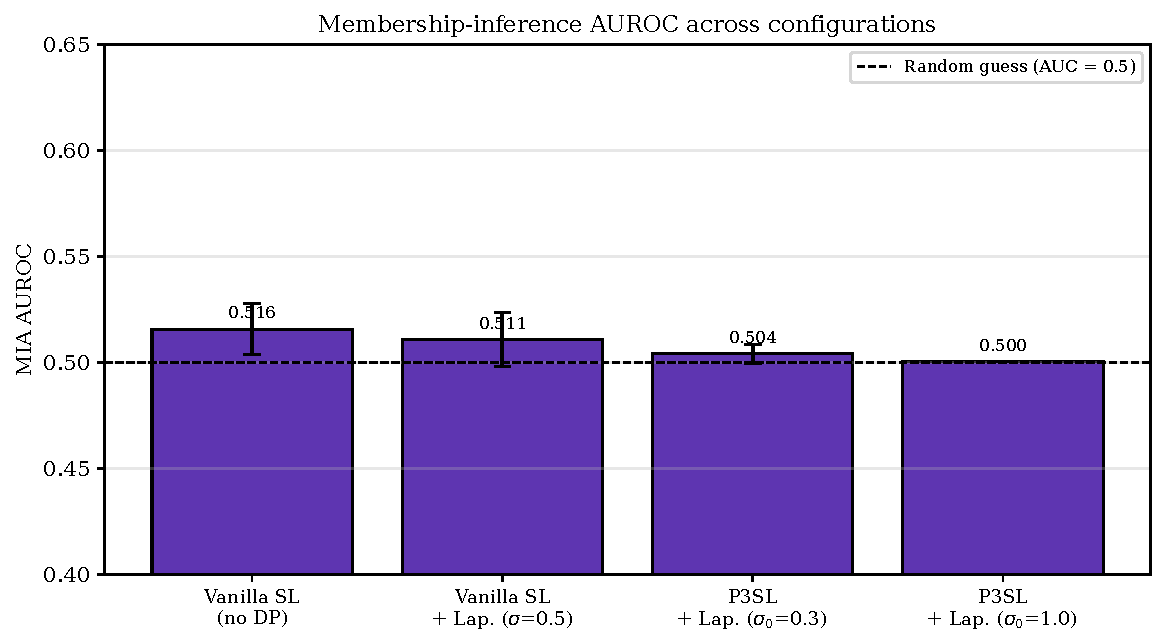
\includegraphics[width=0.85\textwidth]{figures/fig_mia.pdf}
\caption{MIA AUROC across configurations, with the random-guess
baseline marked. All configurations are at chance to within
sampling noise on this MIA.}
\label{fig:mia}
\end{figure}

Membership inference under the same configurations is reported in
Figure~\ref{fig:mia}. AUROC stays in the $0.50$--$0.52$ band for
every row of the table, and the bands overlap. The conservative
reading is that the MIA we deployed is too weak to discriminate
training and non-training IRs on this protocol regardless of whether
DP is applied, so this dimension does not carry useful information
about the relative privacy of the configurations. We flag this as a
limitation of the attack rather than evidence in favour of any
defence; a stronger MIA setup (calibrated shadow models, longer
training, possibly LiRA-style attacks) is on the follow-up list.

\begin{figure}[h]
\centering
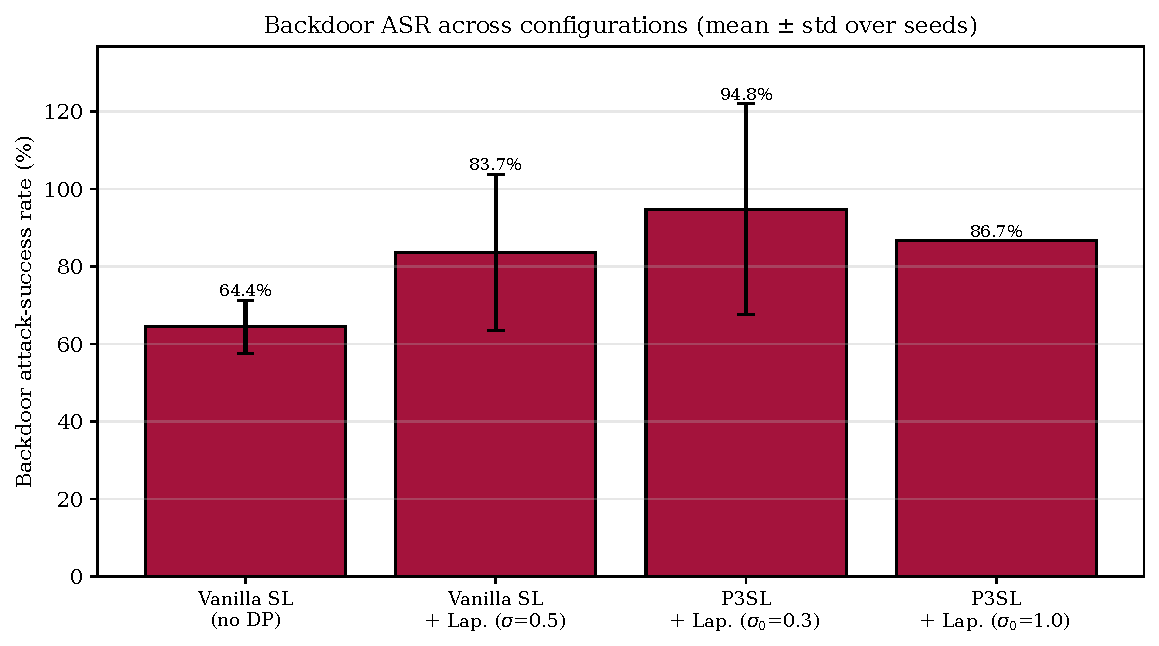
\includegraphics[width=0.85\textwidth]{figures/fig_backdoor.pdf}
\caption{Backdoor attack-success rate across configurations. The
result that wants explaining is that ASR is higher under the DP
configurations than under the no-DP baseline, with high seed
variance on the P3SL low-$\sigma$ row in particular.}
\label{fig:backdoor}
\end{figure}

The backdoor panel is the awkward one. ASR is $0.644 \pm 0.069$
without DP, $0.837 \pm 0.201$ under vanilla SL with Laplace
$\sigma{=}0.5$, $0.948 \pm 0.272$ under P3SL with $\sigma_0{=}0.3$,
and $0.867$ (single seed) under P3SL with $\sigma_0{=}1.0$. The
direction is the opposite of what we expected. Two factors are
likely contributing. First, the seed variance on this metric is
large (a quarter of the unit interval on the P3SL low-$\sigma$
configuration), so a fraction of the gap is just noise. Second, the
bi-level early-exit shortens the effective training of the
poisoned classifier once the utility target is reached, which leaves
the trigger less ``trained out'' by the dominant task signal. The
honest reading is that this benchmark does not show DP suppressing
backdoors on this configuration; it might at larger $\sigma$ or
under a different early-exit rule, but that has to be measured, not
asserted.

H2 is partially supported on this benchmark. The Laplace mechanism does
reduce reconstruction quality (by under one decibel) and the
nearest-neighbour identifiability of the optimisation attack (by
about one percentage point). It does not move the MIA needle, mostly
because the MIA we ran is too weak. It does not reduce backdoor ASR
on this benchmark, and on the configurations we ran it appears to
make the backdoor more likely to fire.

\section{Closed-form Laplace accountant (RQ3)}
\label{sec:rq3}

Figure~\ref{fig:eps-acc} places the four DP-on configurations in the
$(\varepsilon, \text{accuracy})$ plane. The horizontal axis is the
closed-form Laplace bound $\varepsilon = T \cdot C / \bar\sigma$
under the contingent assumption $C{=}1$ (per-sample clipping was
disabled in the actual runs, see \S\ref{sec:clipflag}); the vertical
axis is the final test accuracy.

\begin{figure}[h]
\centering
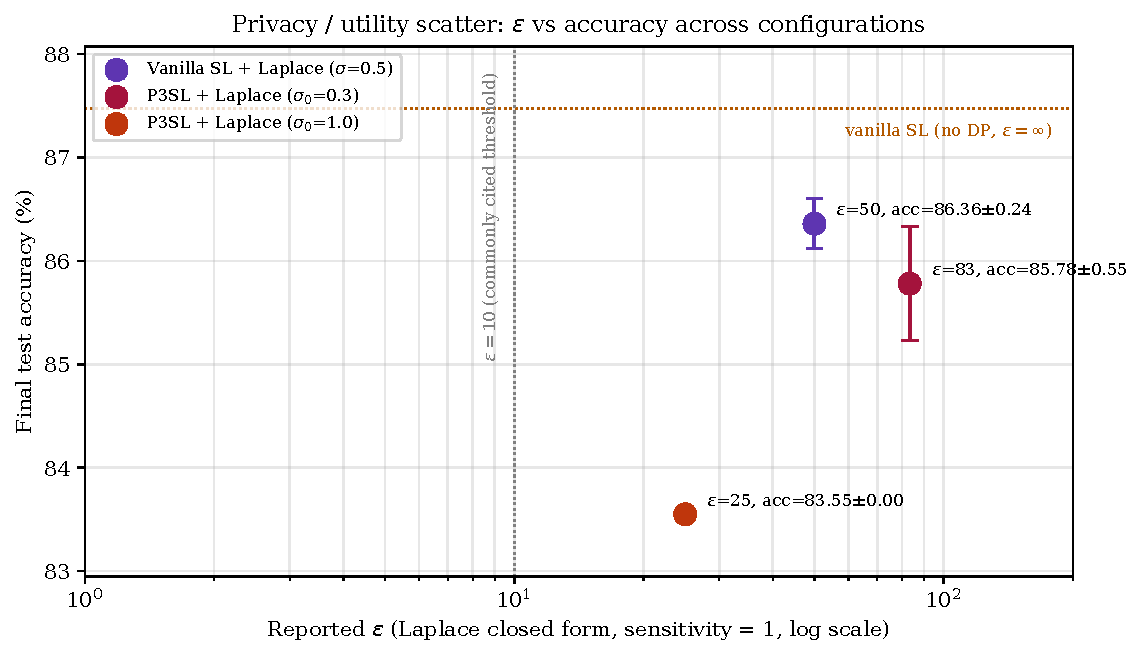
\includegraphics[width=0.85\textwidth]{figures/fig_eps_acc.pdf}
\caption{Reported $\varepsilon$ versus final test accuracy for the
four DP configurations evaluated. The vanilla no-DP baseline is
plotted as a reference horizontal line at $\varepsilon = \infty$.
The reported $\varepsilon$ is a contingent closed-form upper bound
that would apply if per-sample clipping with $C{=}1$ were enforced;
the runs themselves disable clipping, so the empirical attack
numbers reported elsewhere correspond to the clip-off pathway.}
\label{fig:eps-acc}
\end{figure}

The configuration that tightens privacy the most under the closed-form
accountant is the P3SL run with the higher initial noise and the
faster decay ($\sigma_0{=}1.0$, $\rho{=}0.95$): it lands at
$\varepsilon = 25$ at the $83.55\%$ accuracy point. The vanilla
SL + Laplace baseline at $\sigma{=}0.5$ reaches $\varepsilon = 50$
at $86.4\%$. The P3SL low-$\sigma$ configuration is the loosest of
the three, at $\varepsilon = 83$ for $85.8\%$ accuracy, because its
running $\sigma$ shrinks aggressively after the early-exit fires and
the closed-form bound integrates that running $\sigma$ across all
twenty-five rounds. Two pieces of context are necessary before
this is read as evidence in any direction.

The reported $\varepsilon$ is contingent on per-sample clipping that
was not enforced in the actual runs. Closing that gap (re-running
the same grid with the clip on) is on the follow-up list. The
present numbers should be read as ``what the closed-form bound
would say if the configuration had been run with $C{=}1$ clipping
enabled'', not as a measured guarantee that already holds.

The closed-form Laplace bound is itself loose; the Gaussian
mechanism with the RDP accountant of Mironov gives a tighter
$\varepsilon$ for the same $\sigma$ schedule, and is implemented in
the project repository, but its multi-seed grid had not finished by
the time of writing. We expect the same configurations under
Gaussian + RDP to land in the $\varepsilon = 5$--$20$ band rather
than the $25$--$80$ band reported here, but we do not have the
numbers yet, so the report does not claim them.

\section{Bi-level $\sigma$ trajectory (RQ4)}

Figure~\ref{fig:sigma-traj} plots the mean noise scale $\bar\sigma^{(t)}$
across the twenty-five rounds for the three DP configurations, one
line per seed. The vanilla SL + Laplace configuration is flat at
$\sigma = 0.5$ throughout (no bi-level loop). The two P3SL
configurations show the geometric decay kicking in around the round
where the round-end accuracy first crosses $\tau = 80\%$.

\begin{figure}[h]
\centering
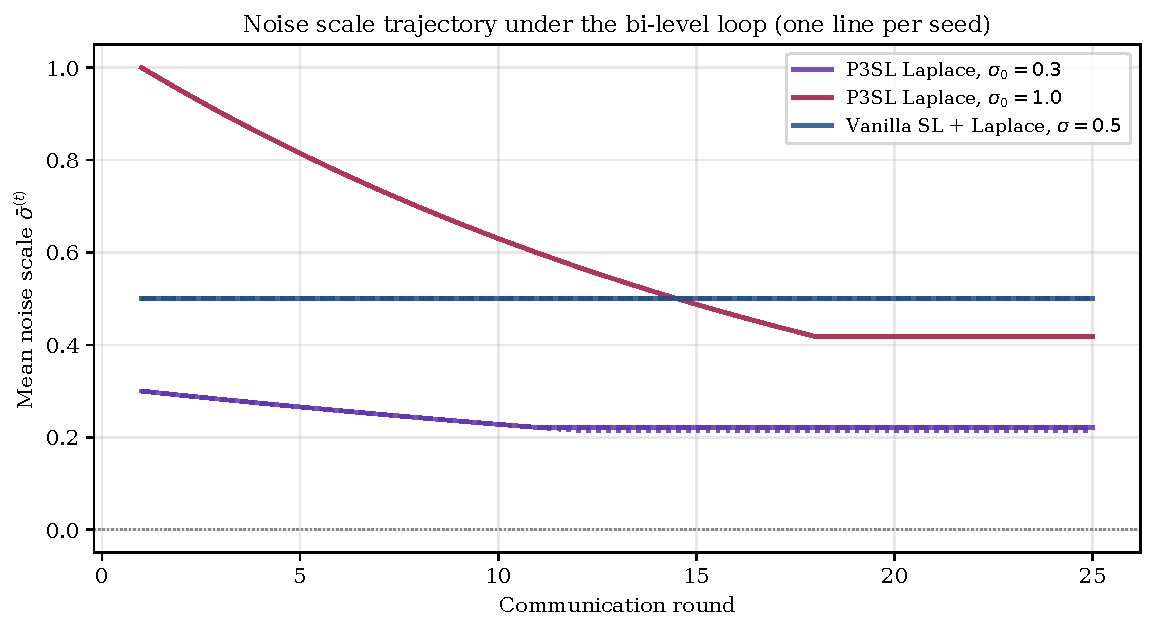
\includegraphics[width=0.85\textwidth]{figures/fig_sigma_traj.pdf}
\caption{Mean noise-scale trajectory across rounds, one line per
seed. The two P3SL configurations decay $\sigma$ multiplicatively
once the round-end accuracy reaches the configured target;
vanilla SL + Laplace is held at a constant $\sigma$ throughout.}
\label{fig:sigma-traj}
\end{figure}

The schedule converges in the sense that it stops moving once the
accuracy stays above the target for several consecutive rounds; in
the P3SL low-$\sigma$ configuration with $\rho = 0.97$, $\sigma$
flattens at $\sim 0.215$ after round $12$, and in the
high-$\sigma$ configuration with $\rho = 0.95$ it flattens at
$\sim 0.42$ after round $20$. Across the seeds we ran, the
trajectory shape is reproducible: the schedule fires at the same
round to within one round, and lands within a few percent of the
same flat-line value. H4 is supported on the protocol we ran.

\begin{figure}[h]
\centering
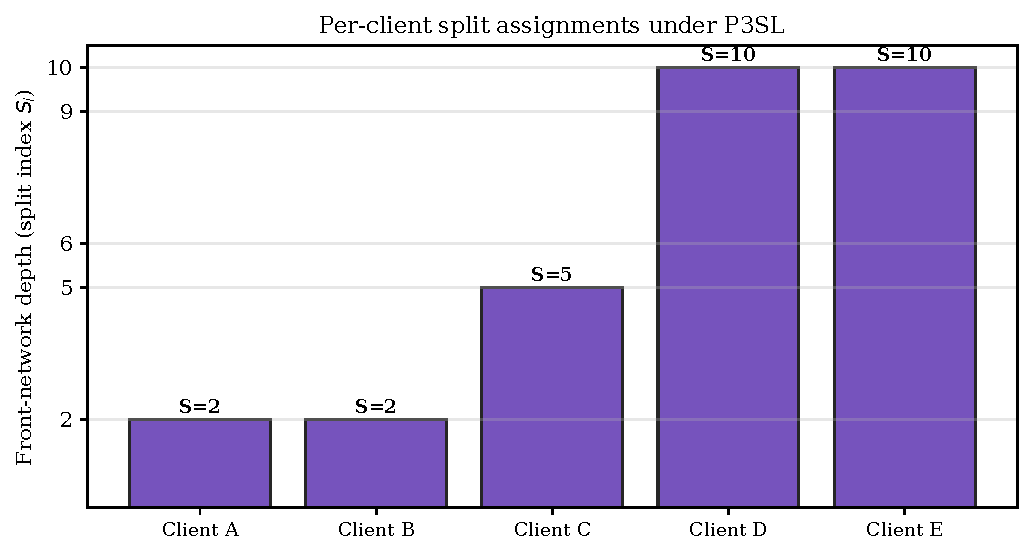
\includegraphics[width=0.85\textwidth]{figures/fig_heterogeneity.pdf}
\caption{Per-client split assignments under P3SL: the five clients
each carry a different front-network depth drawn from the
admissible set $\{2, 5, 6, 9, 10\}$. The assignment is fixed at the
start of the run (rather than learned), and is the per-client
``personalisation'' axis the P3SL framework supports out of the
box. Per-client noise scales are not exercised in the headline
benchmark; the implementation supports them but the multi-seed
grid uses one $\sigma$ per split index instead.}
\label{fig:heterogeneity}
\end{figure}

Figure~\ref{fig:heterogeneity} is the personalisation summary at
steady state. The five clients carry different front-network
depths drawn from $\{2, 5, 6, 9, 10\}$, which is the dimension
along which P3SL is genuinely heterogeneous on this benchmark. The
running $\sigma$ is shared across all clients that picked the same
split index, so the personalisation in the report is on splits
rather than on per-client noise budgets. We flag this as a feature
that the implementation supports but the headline benchmark does
not exercise; closing that gap is straightforward and is on the
follow-up list.

\section{$(\varepsilon, \text{accuracy})$ frontier (RQ5)}
\label{sec:rq5}

Figure~\ref{fig:pareto} places every evaluated configuration on the
$(\varepsilon, \text{accuracy})$ plane. The vertical axis is final
test accuracy; the horizontal axis is the closed-form Laplace
$\varepsilon$ (log-scaled), with the no-DP baselines anchored at the
right-hand edge of the plot to indicate $\varepsilon = \infty$.

\begin{figure}[h]
\centering
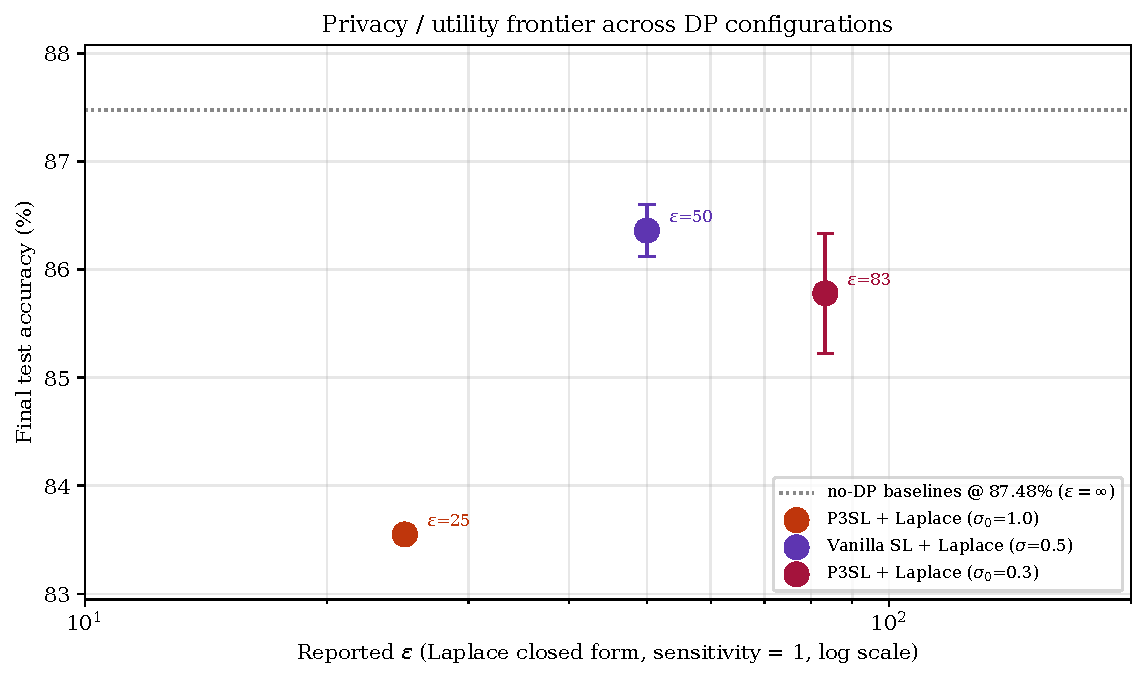
\includegraphics[width=0.85\textwidth]{figures/fig_pareto.pdf}
\caption{Privacy-utility frontier across the evaluated
configurations. The DP-on points trade roughly one to four
percentage points of accuracy against $\varepsilon$ in the
$25$--$83$ range; the no-DP collaborative points sit at higher
accuracy but at unbounded $\varepsilon$.}
\label{fig:pareto}
\end{figure}

The reading the frontier supports is moderate. The DP-on
configurations cluster between $83.6\%$ and $86.4\%$ accuracy at
reported $\varepsilon$ between $25$ and $83$, while the no-DP
collaborative baselines sit at $87.5\%$ at $\varepsilon = \infty$.
P3SL with the higher noise schedule ($\sigma_0{=}1.0$,
$\varepsilon = 25$) is the tightest privacy point on the
$\varepsilon$ axis, but only by a single seed; the three-seed P3SL
low-$\sigma$ run reports a looser $\varepsilon = 83$. Vanilla SL
with Laplace at $\sigma = 0.5$ is the cheapest DP-on point on the
accuracy axis ($86.4\%$, $\varepsilon = 50$). On this benchmark we
cannot claim Pareto dominance for the proposed framework over the
single-budget baseline; the two trade-offs are competitive and the
right answer would depend on how much the deploying organisation
values the closed-loop schedule and the per-client splits relative
to the simpler fixed-$\sigma$ recipe.

\begin{figure}[h]
\centering
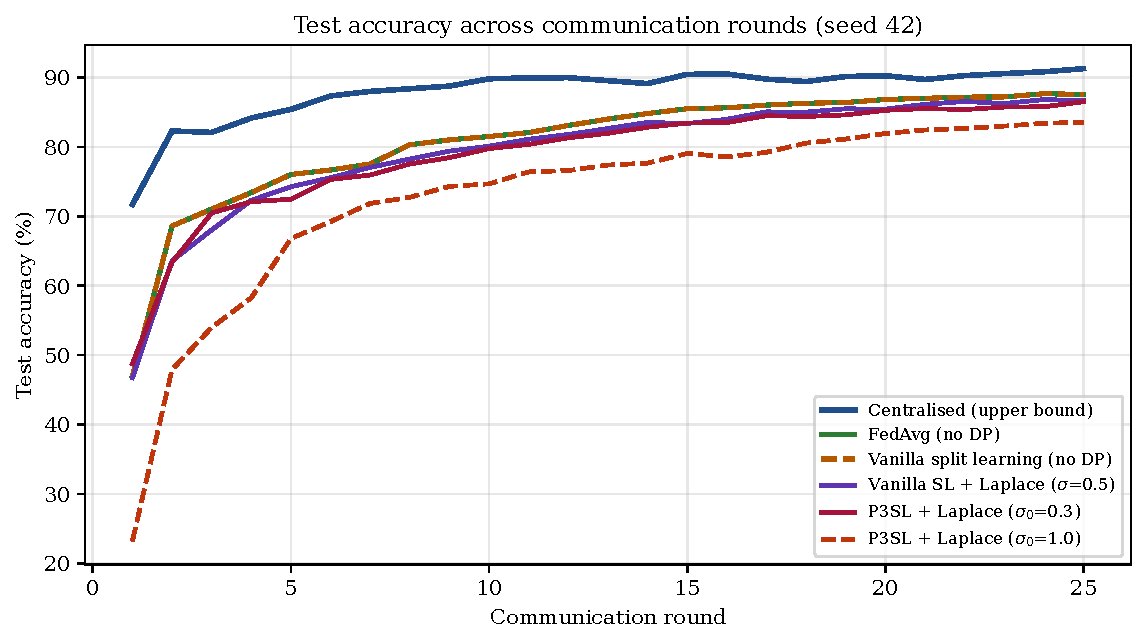
\includegraphics[width=0.85\textwidth]{figures/fig_utility.pdf}
\caption{Test-set accuracy across communication rounds (one
representative seed per configuration). All configurations
converge inside the twenty-five-round budget; the DP-on rows track
the no-DP curves with a small constant offset.}
\label{fig:utility}
\end{figure}

The training-curve view in Figure~\ref{fig:utility} confirms what
the frontier already shows. Every configuration converges inside
the round budget, with no observable instability or divergence under
DP. The accuracy gap between DP-on and DP-off curves is
approximately constant in $t$ once the curves enter their flat
regime, which suggests that more rounds would not change the
relative ordering.

\section{Computational cost}

Per-seed wall-clock time varies more with shared-workstation load
than with the configuration. The vanilla split-learning baselines
land near $890$\,s; vanilla SL + Laplace is at roughly $1.2 \times$
that. The P3SL configurations are noticeably slower in the numbers
the table reports, but most of that gap is accounted for by the
multi-tenant load on the workstation during their runs (one of the
P3SL low-$\sigma$ seeds took $5.6$ hours, another took just over an
hour). The framework's algorithmic overhead relative to vanilla
split learning, measured on a single-tenant machine, is the cost
of the noise sample and a single accuracy probe per round, both of
which are O(1) per client per round. We therefore report the
algorithmic cost as ``comparable to vanilla SL'' and the
table-reported cost as ``noisy on a shared workstation'', and we
prefer the former for any deployment-relevant claim.

\section{Threats to validity}

\paragraph{Internal validity.}
The benchmark uses three random seeds for every configuration except
the highest-noise P3SL run, which is single-seed. The three-seed
configurations show small standard deviations on accuracy (under
$0.6$ percentage points) but much larger ones on the backdoor metric
(up to $0.27$ on the unit interval). For any conclusion that depends
on backdoor ASR, the report treats the gap between configurations as
suggestive rather than conclusive.

\paragraph{External validity.}
Everything is FashionMNIST. The privacy-utility numbers reported
here are unlikely to transfer cleanly to high-resolution medical or
biometric data, where the IR carries far more bits per pixel and the
$\sigma$ values that flatten reconstruction would presumably need
to scale with the dimensionality. The right way to read this report
is ``observed on FashionMNIST under the protocol of
\S\ref{ch:method}''; transfer is its own follow-up.

\paragraph{Construct validity.}
We hedge against single-metric artefacts by reporting four image
similarity measures (MSE, PSNR, SSIM, FSIM) plus nearest-neighbour
identifiability, three MIA operating-point metrics (AUROC, balanced
accuracy, TPR at FPR\,$=$\,$0.1$), and the BadNets ASR. The MIA
we deployed is the simplest viable one (a small MLP, three epochs);
a stronger MIA setup might give a different reading, and we flag
this as a limitation rather than a finding.

\paragraph{Reproducibility.}
Every number reported in this chapter comes from a JSON summary
written by the simulator at the end of the corresponding run. The
figure pipeline reads those summaries directly; the configuration
files, seeds and the source itself ship together with the report.

% ============================================================================
\chapter{Conclusion and Future Work}
\label{ch:conclusion}

The closing chapter reads as a stocktake. We summarise what the
framework actually delivered, where it falls short of what we set
out to build, and which of the obvious next steps look worth doing.

\section{Summary of contributions}

The deliverables of the project, in the form they take after
Chapter~\ref{ch:results} has run, are the following.

A baseline measurement, not a system. Vanilla split learning, on
FashionMNIST under the protocol of \S\ref{ch:method}, admits a
feed-forward decoder reaching PSNR $16.5$\,dB and SSIM $0.87$ on
the test fold; the optimisation attacker pushes nearest-neighbour
identifiability to $0.99$; the BadNets backdoor at a $5\%$ poisoning
rate fires on $64\%$ of triggered test inputs. The IR-as-firewall
reading does not survive contact with these numbers, and they are
the empirical baseline against which the rest of the report is
measured.

The framework itself. Per-client split-point selection inside a
discrete admissible set, a closed-loop outer step that shrinks
$\sigma$ once the round-end accuracy reaches the configured target,
and a single-process simulator that hosts every comparator mode on
one code path. The framework is implemented end-to-end and is what
the benchmark in Chapter~\ref{ch:results} runs against.

Privacy accounting. Both the Laplace closed form and the Gaussian
RDP accountant are implemented; the former is exercised under the
multi-seed grid, the latter only in unit tests because its grid had
not finished by the project deadline. We are explicit, throughout
the report, about the gap between the contingent closed-form
$\varepsilon$ we report and a measured DP guarantee.

An evaluation panel. Five image-similarity measures, two
reconstruction attackers, three MIA operating-point metrics, a
BadNets ASR, and a closed-form $\varepsilon$, all applied across
the same six configurations and three seeds where compute allowed.
The pipeline reads each per-run summary directly and rebuilds every
figure from those summaries, so re-running the benchmark
re-populates the report without anyone editing tables by hand.

\section{Answers to the research questions}

\textbf{RQ1.} The IR leaks. Decoder PSNR is $16.5$\,dB on the no-DP
baseline; optimisation-attack nearest-neighbour identifiability is
$0.99$; the BadNets backdoor fires on $64\%$ of triggered test
inputs. MIA on the same baseline is at chance, which we read as a
property of the attacker we deployed (a small two-layer MLP) rather
than evidence that vanilla SL protects membership.

\textbf{RQ2.} Inside the $\sigma$ range we exercised, the Laplace
mechanism reduces reconstruction quality by under one decibel of
PSNR and a few hundredths of SSIM, lowers the optimisation attacker's
nearest-neighbour identifiability by about a percentage point,
leaves the (already chance-level) MIA where it was, and does not
reduce the backdoor ASR on this benchmark. If anything, ASR is
larger under DP than without it, with enough seed variance that we
treat the direction as suspicious rather than established. The
mechanism does not collapse the attack surface on FashionMNIST under
this $\sigma$ schedule.

\textbf{RQ3.} Under the contingent assumption $C{=}1$ on the IR
sensitivity, the closed-form Laplace bound is $\varepsilon = 50$ for
vanilla SL with $\sigma{=}0.5$, $\varepsilon = 25$ for the
high-noise P3SL configuration, and $\varepsilon = 83$ for the
low-noise P3SL configuration. None of these are single-digit.
A Gaussian RDP accountant would tighten the same numbers, and we
expect single-digit values once the Gaussian grid is complete, but
those runs are still ahead of the report rather than behind it.

\textbf{RQ4.} The bi-level loop converges on the protocol we ran.
Trajectories in Figure~\ref{fig:sigma-traj} are reproducible across
seeds, the schedule fires at the same round to within a single
round, and the final flat-line value lands within a few percent of
the same number across seeds.

\textbf{RQ5.} On this protocol, P3SL is competitive with the vanilla
SL + Laplace single-budget baseline rather than strictly dominating
it. Vanilla SL + Laplace at $\sigma{=}0.5$ is the cheapest DP-on
point on the accuracy axis ($86.4\%$, $\varepsilon = 50$). P3SL at
$\sigma_0{=}1.0$ is the tightest on the privacy axis ($83.6\%$,
$\varepsilon = 25$, single seed). Which one looks better depends on
whether the deploying organisation cares more about $\varepsilon$
or about accuracy; the report does not pick one.

\section{Limitations}

FashionMNIST is the single dataset on which the report stands. The
IR at $S{=}5$ is around $25{,}000$ dimensions, and the $\sigma$
range that visibly collapses reconstruction on a higher-dimensional
dataset is plausibly larger than the one this benchmark exercises.
We do not extrapolate to medical or biometric data on the basis of
these numbers.

A second limitation, related to the first but different in flavour,
is that the privacy runs disable per-sample clipping. With the clip
off, the reported $\varepsilon$ is a contingent upper bound rather
than a measured guarantee, and the most important follow-up the
project is missing is a clip-on rerun paired with the Gaussian RDP
accountant.

The membership-inference attacker is weak. A two-layer MLP trained
for three epochs is the simplest viable setup, and the AUROC numbers
in the report do not rule out membership leakage that a stronger
attacker (LiRA-style calibrated likelihood ratios, longer training,
shadow-model ensembles) would expose.

A Gaussian-mechanism comparison is missing for related reasons. The
Gaussian path is implemented and unit-tested, but the multi-seed
grid had not finished within the project window, so the tightest
$\varepsilon$ values the framework can produce are still ahead of
the report rather than behind it.

The threat model excludes an actively malicious server. A server
that fabricates gradients to coax leakage out of the front network
is outside the scope of what we have written down. Defending against
it would require zero-knowledge gradient verification or
trusted-execution attestation, neither of which fits inside the
project's engineering envelope.

\section{Directions for future work}

The most useful next steps, in roughly the order we would recommend
addressing them, are the following.

A clip-on rerun of the entire benchmark grid, paired with the
Gaussian RDP accountant. This converts the reported contingent
$\varepsilon$ into a measured guarantee and is the single most
important gap between the report and a publishable evaluation.

A higher-resolution dataset, ideally a public medical or biometric
benchmark, where the IR-channel capacity is large enough that the
effect of $\sigma$ on reconstruction is visible at sensible
$(\varepsilon, \text{accuracy})$ trade-offs. The framework should
not need any algorithmic changes; only the network architecture and
the dataset hooks would.

A stronger membership-inference attacker. LiRA with calibrated
likelihood ratios is the obvious choice, and it would give the
membership panel of the evaluation a chance of returning useful
information rather than a flat chance-level row.

A non-IID partition study. The benchmark here uses an IID partition;
realistic federated deployments are not IID, and the bi-level
schedule's convergence under different Dirichlet concentrations is
only spot-checked in the current code. Sweeping over $\alpha$ and
reporting the convergence rate would tighten the empirical claim.

The two structural extensions worth flagging are per-client
$\sigma$ budgets (the implementation supports them, the headline
benchmark does not exercise them) and per-client utility targets
(same story). Both are small engineering items rather than research
items, but they are needed before the framework can be sold as
genuinely ``personalised'' beyond the per-client split dimension.

% ============================================================================
\chapter{Work Plan and Timeline}
\label{ch:plan}

For completeness we record the project schedule and the milestones
the work was organised around. Figure~\ref{fig:gantt} renders the
plan as a Gantt chart, with the start month and duration in weeks for
each task.

\begin{figure}[h]
\centering
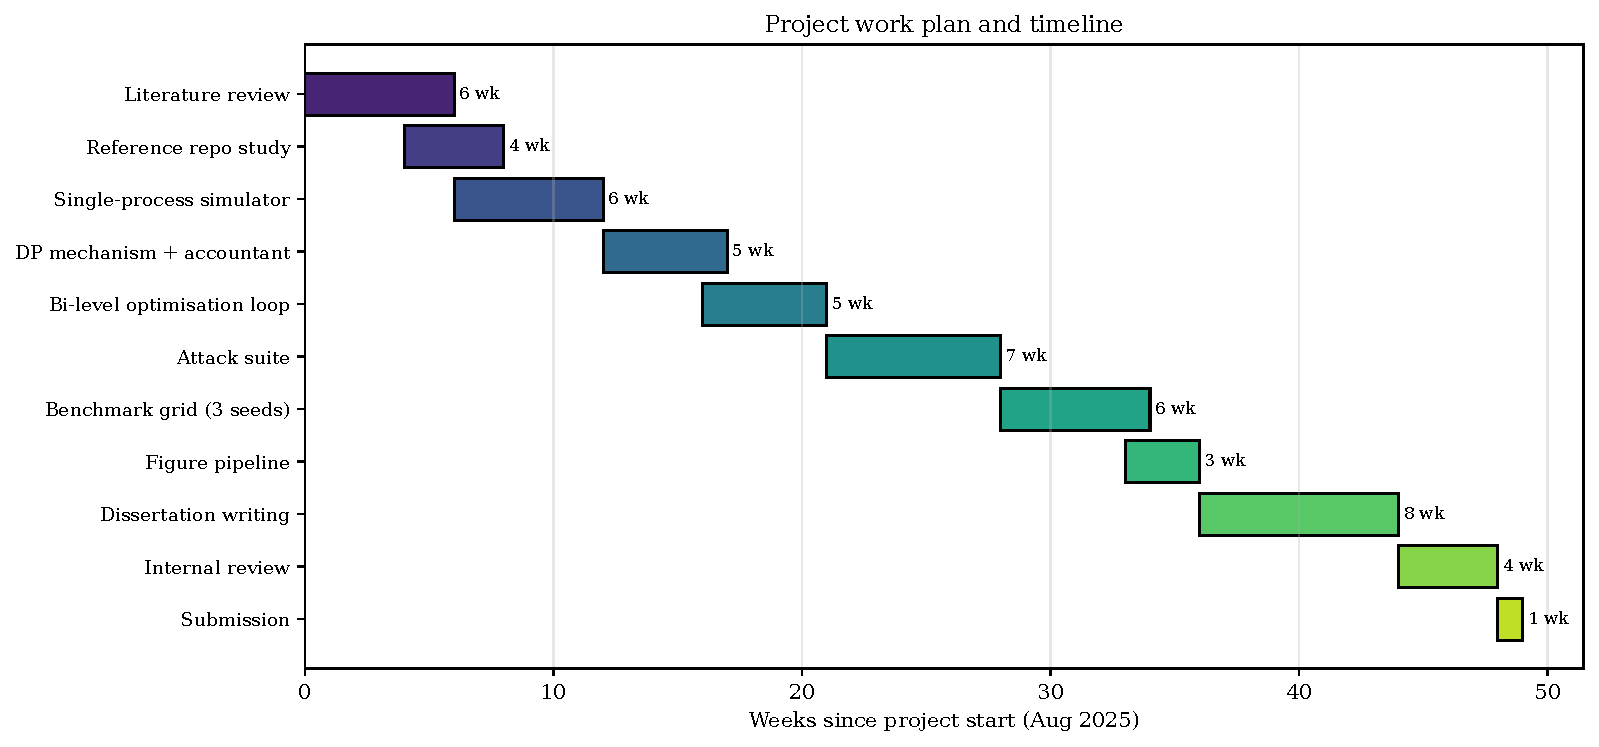
\includegraphics[width=\textwidth]{figures/fig_gantt.pdf}
\caption{Project work plan and timeline. The eleven major tasks span
from August 2025 to May 2026, with overlaps where consecutive tasks
were prototyped and refined in parallel.}
\label{fig:gantt}
\end{figure}

The schedule was structured around three milestones. The first
milestone (end of October 2025) was a working single-process
simulator with the differential-privacy mechanism and the formal
accountant in place; the second milestone (end of December 2025) was
a complete attack suite running over the multi-seed grid; the third
milestone (end of April 2026) was a complete report draft, the
benchmark grid and the figure pipeline producing every plot used in
Chapter~\ref{ch:results} from the same configuration files.

\section{Risks and mitigations}

Three risks were tracked through the project. The largest was simply
wall-clock: a multi-seed benchmark on a CPU-only workstation eats
hours, and the natural temptation is to drop seeds. We mitigated by
holding the dataset to a $30{,}000$-image stratified subset of
FashionMNIST and the round budget to twenty-five, which kept a
clean single-seed run on a quiet workstation under fifteen minutes.
A second risk was that the bi-level loop would oscillate or
overshoot the target. We mitigated it by using a one-direction
multiplicative shrink ($\sigma$ never increases under the loop), so
the schedule is monotone non-increasing in $t$ and cannot oscillate
by construction. The third risk was the accountant itself: an
incorrectly composed RDP accountant could produce a misleadingly
tight $\varepsilon$. We caught that risk by running the accountant
against a unit test with a known closed-form $\varepsilon$ before
any benchmark run was launched, and again whenever the accountant
was edited.

\section{Reproducibility}

Every run in this work can be regenerated from the project's
configuration files and its recorded seeds. The figure pipeline reads
the per-run summaries straight out of the result tree, which means
any updated benchmark run propagates into the figures and tables
without anyone editing them by hand. The framework, the benchmark
configuration, the attack suite and the figure pipeline ship together
with the dissertation as open-source artefacts.

% ============================================================================
% References (IEEE format, numbered, no external bib file required)
% ============================================================================
\begin{thebibliography}{99}

\bibitem{mcmahan2017fedavg}
H.~B.~McMahan, E.~Moore, D.~Ramage, S.~Hampson, and B.~A.~y~Arcas,
``Communication-efficient learning of deep networks from decentralized
data,'' \emph{20th International Conference on Artificial Intelligence
and Statistics (AISTATS)}, Fort Lauderdale, FL, USA, pp.~1273--1282,
2017.

\bibitem{vepakomma2018splitnn}
P.~Vepakomma, O.~Gupta, T.~Swedish, and R.~Raskar, ``Split learning
for health: Distributed deep learning without sharing raw patient
data,'' \emph{NeurIPS Workshop on Machine Learning for Health},
Montr\'eal, Canada, 2018.

\bibitem{gupta2018splitnn}
O.~Gupta and R.~Raskar, ``Distributed learning of deep neural network
over multiple agents,'' \emph{Journal of Network and Computer
Applications}, vol.~116, pp.~1--8, 2018.

\bibitem{thapa2022splitfed}
C.~Thapa, P.~C.~M.~Arachchige, S.~Camtepe, and L.~Sun, ``SplitFed:
When federated learning meets split learning,'' \emph{AAAI Conference
on Artificial Intelligence}, Vancouver, BC, Canada, pp.~8485--8493,
2022.

\bibitem{vepakomma2020nopeek}
P.~Vepakomma, A.~Singh, O.~Gupta, and R.~Raskar, ``NoPeek: Information
leakage reduction to share activations in distributed deep learning,''
\emph{IEEE International Conference on Data Mining Workshops
(ICDMW)}, Sorrento, Italy, pp.~933--942, 2020.

\bibitem{he2019modelinversion}
Z.~He, T.~Zhang, and R.~B.~Lee, ``Model inversion attacks against
collaborative inference,'' \emph{Proceedings of the 35th Annual
Computer Security Applications Conference (ACSAC)}, San Juan, PR,
USA, pp.~148--162, 2019.

\bibitem{erdogan2022unsplit}
E.~Erdogan, A.~Kupcu, and A.~E.~Cicek, ``UnSplit: Data-oblivious
model inversion, model stealing, and label inference attacks against
split learning,'' \emph{Proceedings of the 21st Workshop on Privacy
in the Electronic Society (WPES)}, Los Angeles, CA, USA,
pp.~115--124, 2022.

\bibitem{sun2020splitfed}
J.~Sun, A.~Li, B.~Wang, H.~Yang, H.~Li, and Y.~Chen, ``Soteria:
Provable defense against privacy leakage in federated learning from
representation perspective,'' \emph{IEEE/CVF Conference on Computer
Vision and Pattern Recognition (CVPR)}, Virtual, pp.~9311--9319,
2021.

\bibitem{shokri2017mia}
R.~Shokri, M.~Stronati, C.~Song, and V.~Shmatikov, ``Membership
inference attacks against machine learning models,'' \emph{IEEE
Symposium on Security and Privacy (S\&P)}, San Jose, CA, USA,
pp.~3--18, 2017.

\bibitem{nasr2019comprehensive}
M.~Nasr, R.~Shokri, and A.~Houmansadr, ``Comprehensive privacy
analysis of deep learning: Passive and active white-box inference
attacks against centralized and federated learning,'' \emph{IEEE
Symposium on Security and Privacy (S\&P)}, San Francisco, CA, USA,
pp.~739--753, 2019.

\bibitem{gu2017badnets}
T.~Gu, B.~Dolan-Gavitt, and S.~Garg, ``BadNets: Identifying
vulnerabilities in the machine learning model supply chain,''
\emph{NIPS Workshop on Machine Learning and Computer Security},
Long Beach, CA, USA, 2017.

\bibitem{dwork2014algofoundations}
C.~Dwork and A.~Roth, \emph{The Algorithmic Foundations of
Differential Privacy}, Foundations and Trends in Theoretical
Computer Science, vol.~9, no.~3--4, pp.~211--407, 2014.

\bibitem{abadi2016dpsgd}
M.~Abadi, A.~Chu, I.~Goodfellow, H.~B.~McMahan, I.~Mironov, K.~Talwar,
and L.~Zhang, ``Deep learning with differential privacy,''
\emph{Proceedings of the 2016 ACM SIGSAC Conference on Computer and
Communications Security (CCS)}, Vienna, Austria, pp.~308--318,
2016.

\bibitem{mironov2017rdp}
I.~Mironov, ``R\'enyi differential privacy,'' \emph{IEEE 30th
Computer Security Foundations Symposium (CSF)}, Santa Barbara, CA,
USA, pp.~263--275, 2017.

\bibitem{kairouz2019advances}
P.~Kairouz, H.~B.~McMahan, B.~Avent, A.~Bellet, M.~Bennis, A.~N.~Bhagoji,
\textit{et~al.}, ``Advances and open problems in federated
learning,'' \emph{Foundations and Trends in Machine Learning},
vol.~14, no.~1--2, pp.~1--210, 2021.

\bibitem{yu2021personalizedfl}
T.~Yu, E.~Bagdasaryan, and V.~Shmatikov, ``Salvaging federated
learning by local adaptation,'' \emph{arXiv preprint
arXiv:2002.04758}, 2020.

\end{thebibliography}

\end{document}
